\documentclass{ucetd}
\usepackage{subfigure,epsfig,amsfonts}
\usepackage[sort&compress,numbers]{natbib}
\usepackage{amsmath}
\usepackage{amssymb}
\usepackage{amsthm}
\usepackage{braket}
\usepackage{mathrsfs}
% \usepackage{cancel}

\usepackage{sectsty}
\usepackage{float}
\usepackage{graphicx}
\usepackage{color,soul}
% \usepackage[colorinlistoftodos]{todonotes}
\usepackage{lipsum}

% \usepackage{tikz}
% \usepackage{circuitikz}
% \usepackage{tikz-timing}
% \usetikzlibrary{arrows.meta,decorations.pathmorphing,decorations.pathreplacing,positioning,shapes,fadings}

%Modify directory for loading graphics
\graphicspath{{figures/}}
%Extra
\usepackage{filecontents}
\usepackage{bm}
\usepackage{braket}
\usepackage{setspace}
\usepackage{listings}
\usepackage{multicol}
\usepackage{verbatim}
\usepackage{physics}
\usepackage{dsfont}
\usepackage{pdflscape}
\usepackage{adjustbox}
\usepackage{blkarray}
\usepackage{colortbl}
\usepackage{hyperref}
% \usepackage{adjustbox}
% \usepackage{cancel}
\usepackage{rotating}

\renewcommand{\bibname}{References}





%% Use these commands to set biographic information for the title page:
\title{your thesis title here}
\author{your name here}
\department{Pritzker School of Molecular Engineering}
\division{Pritzker School of Molecular Engineering}
\degree{Doctor of Philosophy}
\date{Month and Year of Graduation}  % date of degree awarding, not the date of the defense

%% Use these commands to set a dedication and epigraph text
\dedication{Dedication text}
%\epigraph{Epigraph Text}

\usepackage{caption}
%\captionsetup{font=footnotesize}
\usepackage{pdfpages}

\begin{document}



\maketitle

\makecopyright
\makededication
%\makeepigraph

%% Make the various tables of contents
\tableofcontents
\cleardoublepage
\phantomsection
\listoffigures
\cleardoublepage
\phantomsection
\listoftables
\newpage

\begin{center}
    \textit{This thesis represents the motivations, results, and conclusions from the following works}:
    \\
    \begin{enumerate}

        \item[] 
    \end{enumerate}

\end{center}
\newpage
 
\acknowledgments
\begin{center}
    \textit{XYZ...}
\end{center}

XYZ

\abstract
Abstract


\mainmatter

% Chapter 1

\chapter{Introduction} % Main chapter title

\label{ch:intro} % For referencing the chapter elsewhere, use \ref{Chapter1} 

%----------------------------------------------------------------------------------------

% Define some commands to keep the formatting separated from the content 
\newcommand{\keyword}[1]{\textbf{#1}}
\newcommand{\tabhead}[1]{\textbf{#1}}
\newcommand{\code}[1]{\texttt{#1}}
\newcommand{\file}[1]{\texttt{\bfseries#1}}
\newcommand{\option}[1]{\texttt{\itshape#1}}
\newcommand{\enquote}[1]{``#1"}
%----------------------------------------------------------------------------------------
\section{The Cosmic Microwave Background}
\section{Beam Systematics and their Impacts on Cosmological Constants}
\subsection{Number of Relativistic Species}
\subsection{Other...}
\chapter{Instrument Overview}
\label{ch:instruments}

We are in the age of precision cosmology, and measurements of the CMB spectra continue to improve in sensitivity.  Now, to measure the CMB polarization anisotropies, scientists are pushing forward the sensitivity of the instruments by increasing detector numbers, improving detector sensitivity, and controlling optical systematics, to name a few.  For example, the Atacama Cosmology Telescope (ACT), a ground-based cosmology experiment, used roughly 3000 bolometric detectors.  The Simons Observatory is scaling its detector count up to more than 50,000 bolometric detectors in order to improve mapping speed and sensitivity.  Looking ahead, the CMB-S4 collaboration, the next-generation cosmology project, plans to scale up even further: to roughly 500,000 detectors.  This, along with the many other improvements in instrumentation, aim to detect the smallest signals of the CMB polarization spectra.

In this chapter, I describe two ground-based cosmology experiments covered in this work: the Atacama Cosmology Telescope (ACT), an operational cosmology experiment~\cite{act_inst}, and the Simons Observatory (SO), the next-generation cosmology experiment~\cite{so19}. 

\section{Atacama Cosmology Telescope}
\begin{figure}[ht]
    \centering
    \includegraphics[width=\textwidth]{Figures/Site_Drone_Picture_July_2019.jpeg}
    \caption{The Simons Observatory (SO) and Atacama Cosmology (ACT) site in the Atacama Desert, Chile. The ACT telescope sits within a ground-shield which can be sen in the bottom center.  The outer ground screen protects the telescope from stray light.  The inner co-moving ground-screen further protects the telescope from stray light during observations.}
    \label{fig:act_so_site}
\end{figure}

The full ACT is shown in Figure~\ref{fig:act_site}.  Figure~\ref{fig:act_inst} shows the ray-trace of ACT's off-axis Gregorian geometry with two reflectors which guide photons into the receiver cabin.  Within the receiver cabin, three optics tubes re-simage the Gregorian focus onto the detector arrays~\cite{thornton_2016}.

\begin{figure}
    \centering
    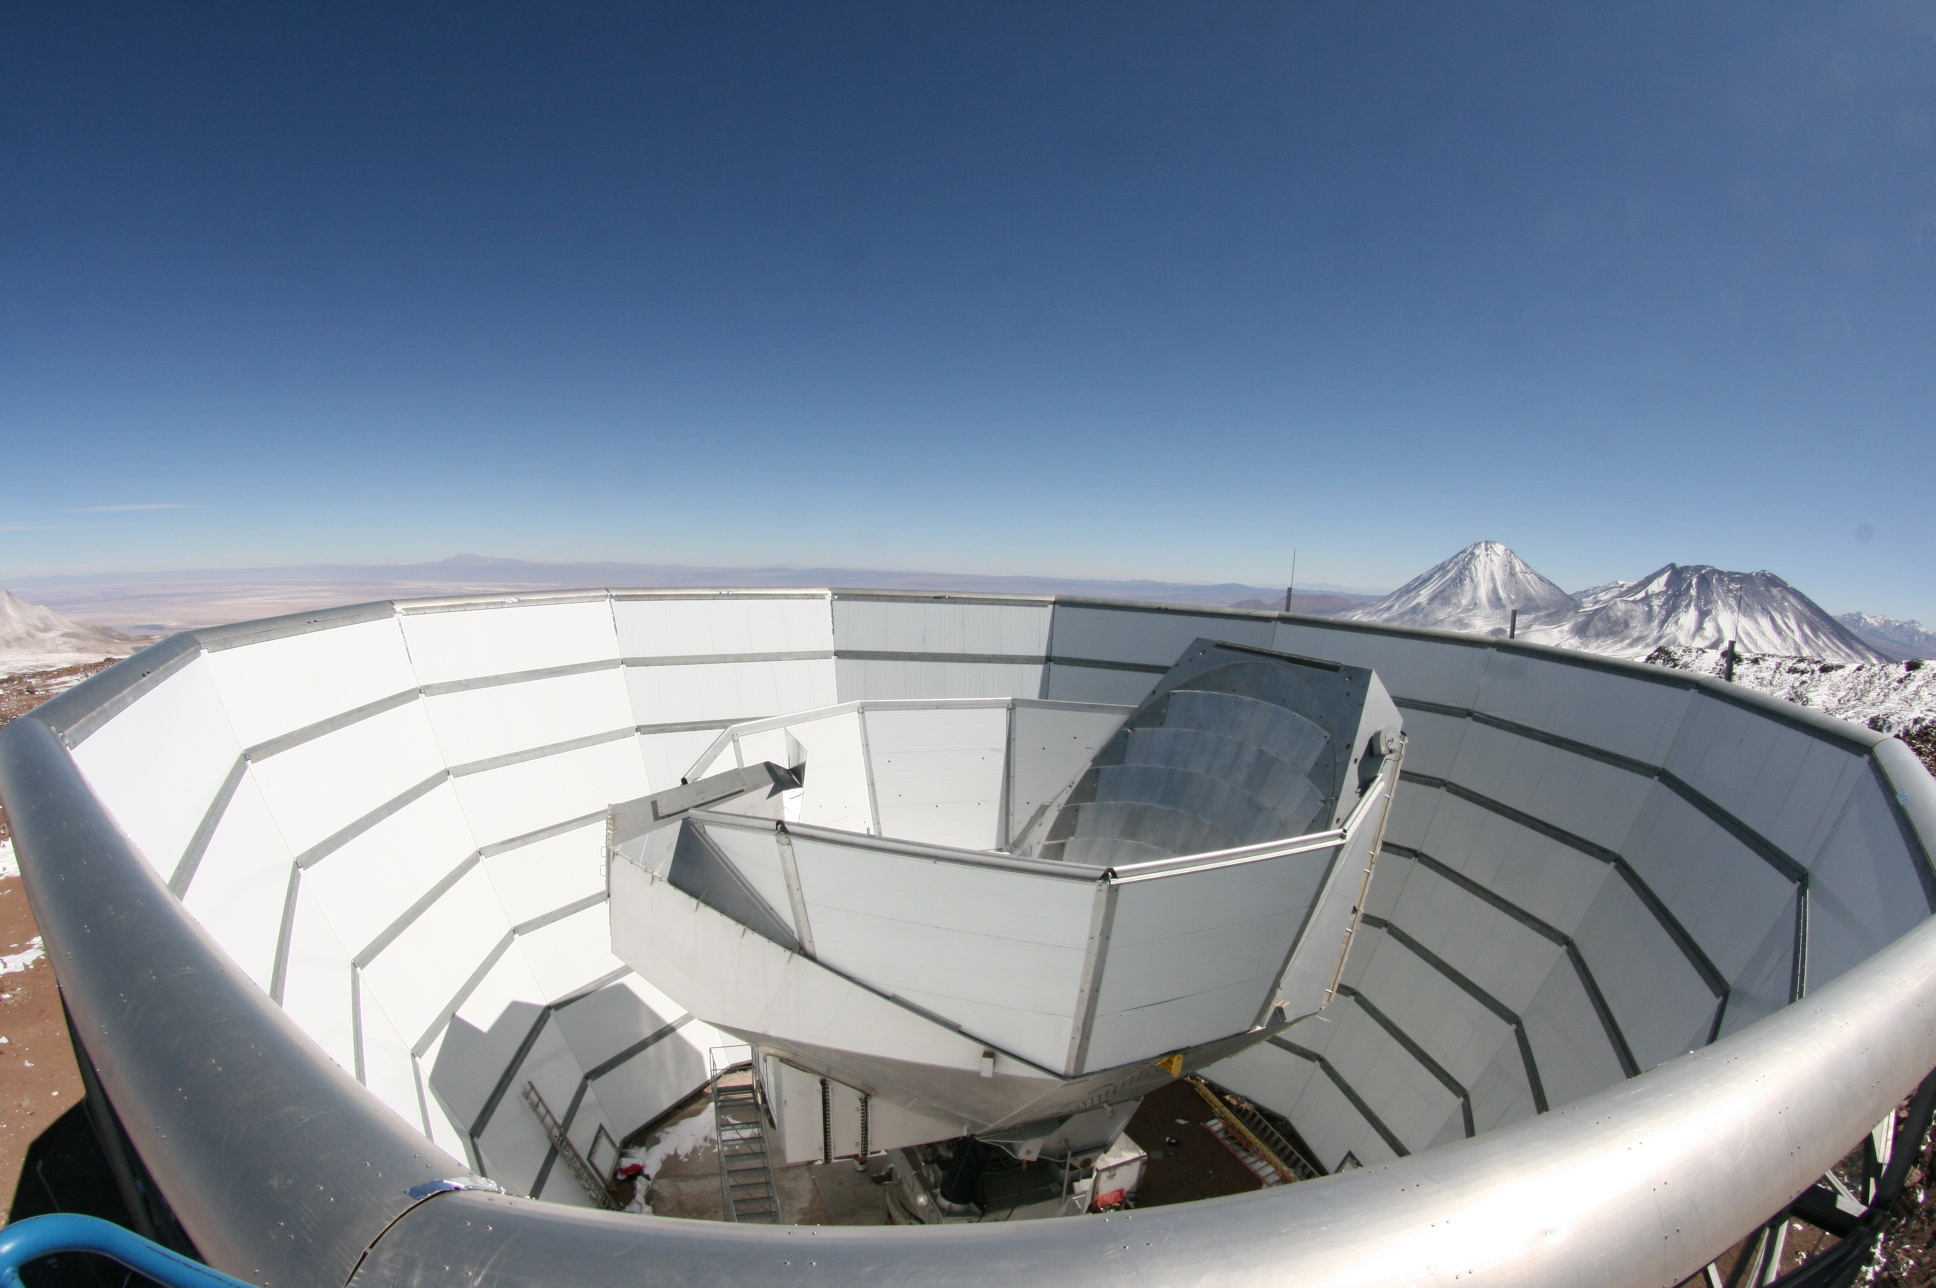
\includegraphics[width = .7\textwidth]{Figures/act_inst_close.jpeg}
    \caption{The Atacama Cosmology Telescope, surrounded by its outer ground screen. The inner co-moving screen further shields the instrument from any stray-light.  One can see the top of the primary mirror behind the co-moving screen.}
    \label{fig:act_site}
\end{figure}

\begin{figure}[t]
    \centering
    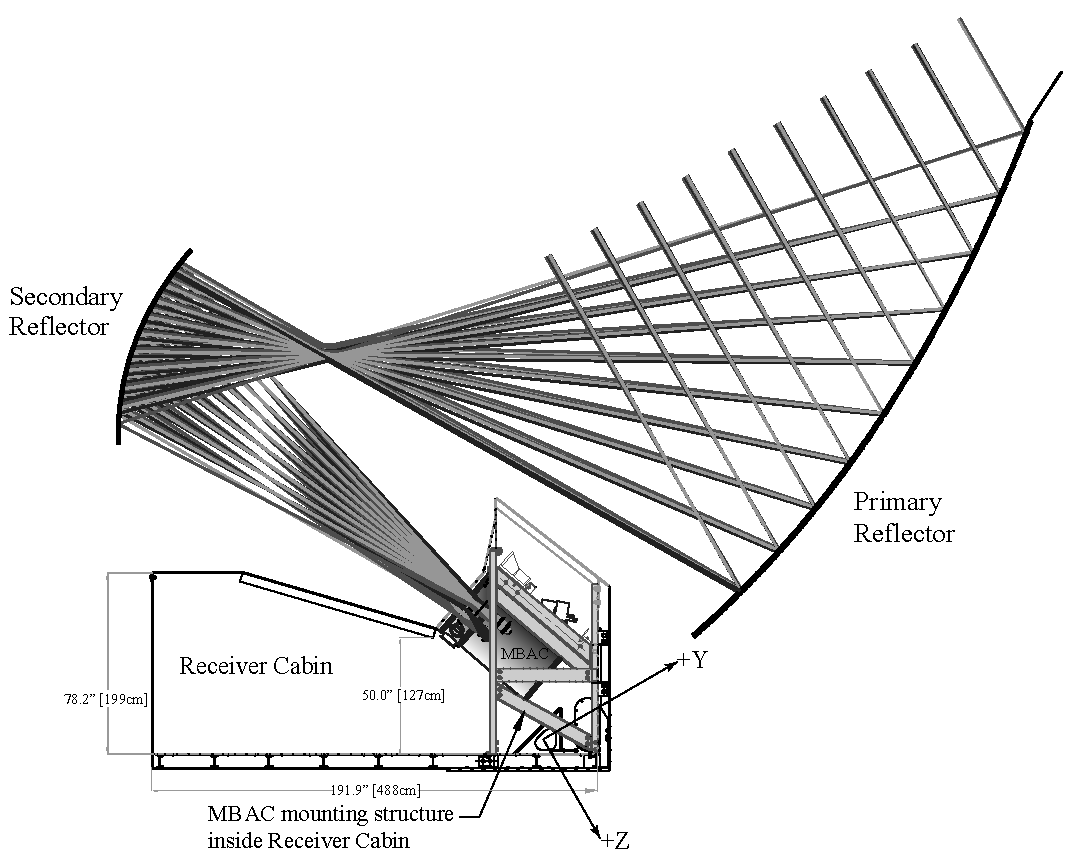
\includegraphics[width = .8\textwidth]{Figures/act_inst.pdf}
    \caption{Ray-trace diagram of the Atacama Cosmology Telescope~\cite{act_inst}.  The telescope is an off-axis Gregorian with two reflectors: the primary is 6\,m in diameter and the secondary 2\,m.  The rays trace into the Millimeter Bolometer Array Camera (MBAC) cryostat which houses the telescope's detectors.}
    \label{fig:act_inst}
\end{figure}

In Chapter~\ref{ch:actbeams} I present the characterization of the ACT beam using point-source stacking.  From the stacking, I also determine polarization leakage in the maps.

\begin{table}[t]
    \centering
    \begin{tabular}{|l|l|l|l|} \hline
        \textbf{ Parameter} &  \textbf{PA4 F150} &  \textbf{PA5 F090}  &  \textbf{PA6 F090}  \\ \hline \hline
        Number of Bolometers & 510 & 510 & 510\\\hline
        Center Frequency (GHz) & 150\,GHz & 90\,GHz & 90\,GHz\\\hline
        Base Temperature & 100\,mK & 100\,mK & 100\,mK\\\hline
        % Angular Resolution & 1 arcmin &1 arcmin &1 arcmin\\\hline
        % Solid Angle & & &\\\hline
        % Sky Coverage & & &\\\hline
    \end{tabular} \caption{ACT Key Characteristics.}
    \label{tab:act}
\end{table}

\section{The Simons Observatory}

SO will test cosmic inflation during the early universe, characterize the primordial perturbations, measure the effective number of relativistic species and the sum of the neutrino masses, and improve our understanding of galaxy evolution and the era of cosmic reionization~\citep{so19,so_science}. 

An ongoing challenge in cosmology instrumentation has been characterizing the polarization spectra of the CMB.  Specifically, the B-mode polarization of the CMB offers a unique window into early-universe physics~\cite{}.  Because scalar perturbations generate E-mode polarization, a measurement of the B-mode polarization directly quantifies the scalar-to-tensor ratio $r$.

The CMB serves as a backlight for large-scale structure, therefore providing insights into gravitational lensing, and ...

The resolution of SO will result in a catalog of extragalactic sources, including active galactic nuclei (AGN), dusty star-forming galaxies, and transient sources including Gamma Ray Burst (GRB) afterglows~\cite{so_science}.  SO expects to catalog 10,000-15,000 AGN sources at flux-densities above 7\,mJy~\cite{Tucci_2011}.  The low frequency coverage of SO will compliment comparison work with other catalogs (e.g. VLA/VLASS, ASKAP/EMU, MeerKAT/MIGHTEE)~\cite{so_science}.  Dusty star-forming galaxies seen by SO will include local galaxies ($z<0.1)$ and high redshift galaxies (approximately $2<z<4$), and strong lensed galaxies beyond this range~\cite{Marrone_2017}.

\begin{figure}[t]
    \centering
    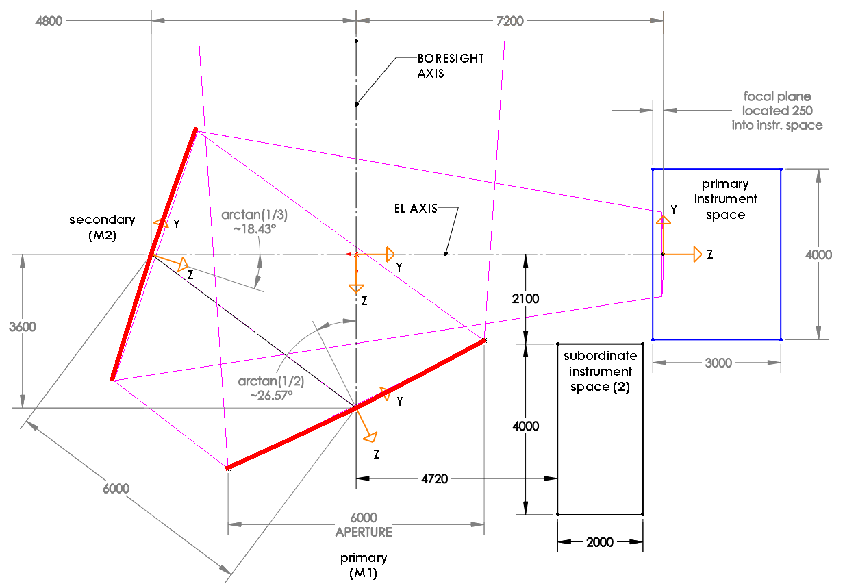
\includegraphics[width = .9\textwidth]{Figures/LAT_rt.pdf}
    \caption{Ray-trace diagram of the Simons Observatory Large Aperture Telescope~\cite{Parshley_2018}.  The telescope is a cross-Dragone with two reflectors, both 6\,m in diameter.  The rays trace into the Large Aperture Telescope Receiver (LATR) cryostat which houses 13 optics tubes.  The optics tubes guide the photons onto the detectors in the focal plane, which are cooled to 100\,mK.}
    \label{fig:so_inst}
\end{figure}

The Simons Observatory (SO) is a series of millimeter-wave telescopes designed to observe the Cosmic Microwave Background (CMB) temperature and polarization signals to an unprecedented sensitivity~\cite{gali18, so19}. With the combination of one Large Aperture Telescope (LAT)~\cite{xu/etal:2020c, zhu18, orlo18, coppi/etal:2018} and three Small Aperture Telescopes (SAT)~\cite{ali20}, the experiment will measure the temperature and polarization anisotropy of the cosmic microwave background with $\sim$\,70,000 background noise limited detectors operating at $\sim$\,100\,mK. 

The Simons Observatory was deployed in the Parque Astronomico located in the Atacama Desert in Chile. The telescope site is situated at an elevation of 5200 meters near the peak of Cerro Toco at $22 ^\circ$ 57' S, $67^\circ$47' W. The arid conditions and elevation at the site minimize contamination to millimeter wave signals from water vapor. 

\begin{table}[ht]
    \centering
    \begin{tabular}{|l|l|l|l|} \hline
        \textbf{ Parameter} &  \textbf{LF} &  \textbf{MF}  &  \textbf{UHF}  \\ \hline \hline
        Number of Bolometers & $>$20,000& $>$20,000& $>$20,000\\\hline
        Base Temperature & 100\,mK & 100\,mK & 100\,mK\\\hline
        Angular Resolution & 1 arcmin &1 arcmin &1 arcmin\\\hline
        Solid Angle & & &\\\hline
        Center Frequency (GHz) & 27-270\,GHz & 27-270\,GHz & 27-270\,GHz\\\hline
    \end{tabular} \caption{SO Key Characteristics.}
    \label{tab:so}
\end{table}

\subsection{Large Aperture Telescope}

The primary mirror is 6\,m in diameter and constructed out of 77 individual adjustable panels, while the secondary mirror is 6\,m in diameter and constructed out of 69 adjustable panels \cite{gali18}.

Figure~\ref{fig:LATR_Cross} shows a cross-section of the LAT Receiver, which houses up to thirteen optics tubes~\cite{Xu_2021}.

Chapter~\ref{ch:ot_holo} presents radio holography measurements of the LAT optics tube, where I characterize the optical performance of the LAT Receiver optics tube.

\subsection{Small Aperture Telescope}

The Small Aperture Telescope (SAT) optical design is a 0.42\,m diameter refractive telescope.  Three SATs will measure the largest angular scales visible from the Atacama Desert.

In Chapter~\ref{ch:sat_holo}, I present radio holography measurements of the SAT optics tube.
\chapter{The Simons Observatory: Characterizing the Large Aperture Telescope Receiver with Radio Holography}
\label{ch:ot_holo}
\section{Introduction}

Simons Observatory (SO) will observe the cosmic microwave background (CMB) temperature and polarization signals using multiple millimeter-wave telescopes~\cite{gali18, so19}.  One Large Aperture Telescope (LAT)~\cite{Niemack:16, Gudmundsson:21,Parshley_2018} and three Small Aperture Telescopes (SAT)~\cite{ali20} together will measure the CMB anisotropies.  SO will provide new constraints on inflationary signals, neutrino mass, and particles beyond the standard model while further improving our understanding of dark energy and galaxy evolution and the era of cosmic reionization~\citep{so19}. 

The LAT is a crossed-Dragone telescope~\cite{6773968,Niemack:16,2021RNAAS...5..100X} developed in collaboration with the Fred Young Sub-millimeter Telescope (FYST)~\cite{ccat,aravena2019ccatprime} Collaboration.  The LAT Receiver (LATR) can hold up to 13 optics tubes, which can accommodate more than 60,000 detectors distributed across 39 detector wafers for CMB studies~\cite{Parshley_2018,zhu2021simons,mccarrick2021simons}.  Each optics tube holds a set of lenses, filters, and baffles which couple light from the telescope onto a set of three polarization sensitive detector arrays.   Realizing the SO science goals depends on achieving stringent sensitivity requirements and controlling systematic effects to be subdominant to the statistical noise.   To achieve this, the optics tubes must have clean beams with well-controlled side-lobe power.  

Testing these aspects of the optics tube performance in the lab is challenging.  Previously, these parameters were verified on ground-based CMB radio telescope systems upon deployment~\cite{alma_holog,2007A&A...465..679N}.  In this paper, we present a new approach to laboratory testing of these systems using the technique of near-field radio holography.  Holography is an instrumentation technique used to measure the complex monochromatic electric field wavefront using the interference between a modulated and non-modulated signal.  Radio holography takes advantage of the antenna theory relationship: the far-field radiation pattern of a reflector antenna is the Fourier Transformation of the field distribution in the aperture plane of the antenna~\cite{alma_holog}.

\begin{figure}[ht]
    \centering
    \includegraphics[width = .8\textwidth]{Figures/lat15.pdf}
    \caption{The Simons Observatory (SO) Large Aperture Telescope (LAT), featuring a segmented primary and secondary mirror.  The mirror's focus is hidden inside the conical baffle near the front of the receiver.  The receiver can hold up to thirteen optics tubes.}
    \label{fig:lat}
\end{figure}

Within radio beam characterization, several techniques exist; 1) scalar beam pattern characterization~\cite{doi:10.1063/1.3292308}, or measuring only the magnitude of the wavefront, 2) vector beam pattern characterization~\cite{2020JLTP..199..156Y,7740846}, or measuring the amplitude and phase of the wavefront, and 3) holographic beam pattern measurement~\cite{387181,7740846}, which we explore here.  While scalar beam pattern characterization requires the beam to be measured at multiple planes along the propagation axis, and vector beam characterization records one complex map, holography records two beam maps (one modulated by the optical element and the other used as a reference) to reconstruct the complex wavefront~\cite{4584681,alma_holog}.

Near-field holography allows us to study the wavefront as it emerges from the optics tube, in the time-reverse sense, from the cryostat.  Using Fresnel diffraction (FD)~\cite{Goodman2005-ne}, these measured fields can be propagated through the optical system to determine the spilled power past the mirrors of the telescope and the far-field beam pattern of the telescope fed by this receiver.  Moreover, these beams are useful for the identification and mitigation of optical problems within the receiver (i.e. optical aberrations, focus, scattered power, etc.).  These measurements enable a detailed verification of system-level optical performance prior to the deployment of a receiver on a telescope.

In Section~\ref{sec:optics_tube} we describe the optical design and components of the SO optics tube.  In Section~\ref{sec:meas_method} we describe the measurement approach including the cryogenic receiver (\ref{sec:meas_method}.\ref{sec:cryo_rec}) and holography hardware (\ref{sec:meas_method}.\ref{sec:meas_hardware}) required for measuring beam maps (full details can be found in Appendix~\ref{app:holog}).  In Section~\ref{sec:results} we present the measured beam maps.   Section~\ref{sec:prop_fields} discusses analysis methods to propagate the measured beams into the far-field using FD.  We present characterization of the optics tube with and without an infrared-blocking filter in Section~\ref{sec:filter}.  Section~\ref{sec:code} details the publicly available code.  We conclude with a discussion of future applications of this approach in Section~\ref{sec:discussion}.  

\section{SO Large Aperture Telescope Optics Tubes Design}
\label{sec:optics_tube}

The LAT is a crossed-Dragone telescope with a 6\,m pupil diameter (Fig.~\ref{fig:lat}).  The LAT Receiver is designed to house thirteen optics tubes, which guide photons onto cryogenic detectors.  These optics tubes must maintain excellent beam quality while also limiting the wide-angle scattering.  The scattering is critical to the ultimate sensitivity of the SO LAT since every percent that is scattered leads to 3\,K of extra noise and a 15(10)\,\% reduction in mapping speed in the 90(150)\,GHz bands which are critical for the SO science.

\begin{figure}
    \centering
    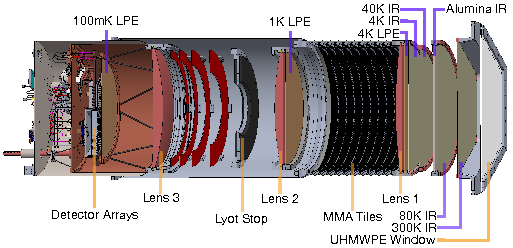
\includegraphics[width = .9\textwidth]{Figures/LATR_OT_Tester_20190221_3.pdf}
    \caption{The Simons Observatory LATR optics tube.  Light enters the optics tube from the right through an ultra-high-molecular-weight polyethylene (UHMWPE) window, and travels through a series of Infrared-Blocking filters (IR), including one alumina IR filter, and passes through the 4\,K Low-Pass Edge mesh filter (LPE). The light is focused on the detector arrays on the left by the three lenses, with two additional LPE filters near the 1\,K and 100\,mK stages.  The components within the optics tube are further described in~\cite{xu/etal:2020c}.}
    \label{fig:latrt}
\end{figure}


Figure~\ref{fig:latrt} shows the LATR optics tube~\cite{xu/etal:2020c}.  Light enters through a 3\,mm thick ultra-high molecular weight polyethylene hexagonal window with an anti-reflection coating~\cite{zhu18}.  Three anti-reflection coated silicon lenses~\cite{Datta:13,golec20} control the beam size and shape, which re-images from the focal plane onto three hexagonal detector wafers.  Each lens is accompanied by a low-pass edge filter (LPE)~\cite{10.1117/12.673162}.  The light is coupled onto the detector wafers using arrays of drilled spline profile feed horns and the polarization is coupled onto the wafer with an orthomode transducer~\cite{10.1117/12.2313405,2022arXiv220104507H}.  Along this path, the light passes through a succession of band-defining and infra-red blocking filters~\cite{10.1117/12.673162}.  From the sky side these are a 300\,K IR blocking filter, an 80\,K IR blocking filter, an 80\,K IR rejecting metamaterial anti-reflection coated alumina filter~\cite{golec20,golec2022}, and a 40\,K IR blocking filter~\cite{10.1117/12.2561720} prior to entering the optics tube.  The filter configuration is described in~\cite{zhu18}.  Between lenses 1 and 2, the walls of the optics tube are coated with baffling metamaterial tiles, described in~\cite{Xu:21}, which control scattering.  The full cold-optical design is described in~\cite{dicker2019cold}.  All optical elements in the optics tube are between 4\,K and 100\,mK.

\section{Measurement Approach}
\label{sec:latot_meas_method}
Here, we describe the hardware and software used in these holography measurements.  Further details can be found in Appendix~\ref{app:holog}.  For this discussion we divide the system into a cryogenic system mounted in the optics tube and a holography system comprised of a source, correlation receiver, and motion system.


\subsection{Cryogenic System}
\label{sec:cryo_rec}
The optics tube is housed in a test cryostat called the LATR tester \cite{Harrington_2020}.  The cryostat holds and cools a single optics tube and provides support for detector readout.  This setup supports up to three detector arrays.   In the test configuration, two are bolometric arrays~\cite{2022arXiv220104507H} and the third is used for the holography measurements. 

The holography array consists of a feedhorn array identical to that used for the bolometric detectors, but with standard wave guide flanges at the outputs. A receiver consisting of a round to rectangular wave guide transition and a harmonic mixer is attached to this feed array.  The mixer was designed to operate from 70-110 GHz, but was found to operate satisfactorily up to 170 GHz. For operational simplicity, we used this mixer over our full frequency range from 80-170\,GHz.% -- though there is some evidence it becomes partially multi-moded towards the upper edge of this range.  
A second identical receiver was also connected for redundancy, but not used in the measurements described here.   Two 0-18\,GHz coaxial connections were made from the receiver to connectors at the cryostat wall.  These coaxes are heat sunk at various stages between the focal plane, which was operated at 4\,K while doing holography, and the 300\,K cryostat wall.  A separate cool down was used to measure the loss along these coaxial feed lines.  The loss  was found to be 23\,dB at the LO frequency (10-13\,GHz).  Accurate knowledge of the loss along the feed lines is critical for providing the correct amount of power to the mixers in the focal plane.  The loss at the interference frequencies (IF) (100\,MHz) is significantly lower and not critical to the function of this system.

\begin{figure}
    \centering
    \includegraphics[width = .95\textwidth]{Figures/LATRt_isometric.pdf}
    \caption{Schematic of holography setup.  Two local oscillators (LO's) supply frequencies ($f_1$ and $f_2 = f_1+f_{\text{offset}}$), one serving as a non-modulated reference signal, while an active multiplier modulates the other.}
    \label{fig:setup}
\end{figure}

\subsection{Holography System}
\label{sec:meas_hardware}

Figure~\ref{fig:setup} shows a schematic overview of the LATR tester (LATRt) holography hardware.  Two millimeter-wave sources are used to measure the full SO MF band: F90 (80-120\,GHz) and F150 (130-170\,GHz).  Only one is mounted at a given time.  These sources are broadcast into the receiver using standard gain feed horns held close to the window (4.5\,cm in F90 and 11.5\,cm in F150 due to the different attenuator waveguide lengths).  We therefore expect different measured beam sizes between the two sets of frequencies, since the beam expands as it leaves the optics tube.
 


A motorized two-dimensional  stage holds the source and is mounted on a support structure above the LATRt.  During a measurement, the source (frequency is fixed) is moved over a $50\times50$\,cm range with 0.25\,cm steps (black arrows in Figure~\ref{fig:setup}).   One map takes roughly 12 hours to complete.

A common local oscillator (LO2 in Figure~\ref{fig:setup}) is fed to two harmonic mixers: 1) picked off from the source and 2) at the output of the cryogenic receiver.  The IF signal from both mixers in the ~0-100\,MHz band is amplified and passed to a digital correlator (Casper ROACH2 ~\cite{roach2}) which computes the complex correlation between the two signals~\cite{ches18}.  The FPGA on the ROACH2 board outputs the amplitude and the phase of the correlated output, subdivided into a number of 100\,kHz wide bins.  Only the bin associated with the IF frequency is used in subsequent analysis.  The software to program and analyze output from the FPGA is made public on the \textit{McMahonCosmologyGroup} GitHub page in a package called \verb|holog-exp|~\cite{holog-exp}.  Appendix~\ref{app:holog} provides further details to the hardware of the holography setup.


\begin{figure*}[ht]
    \centering
    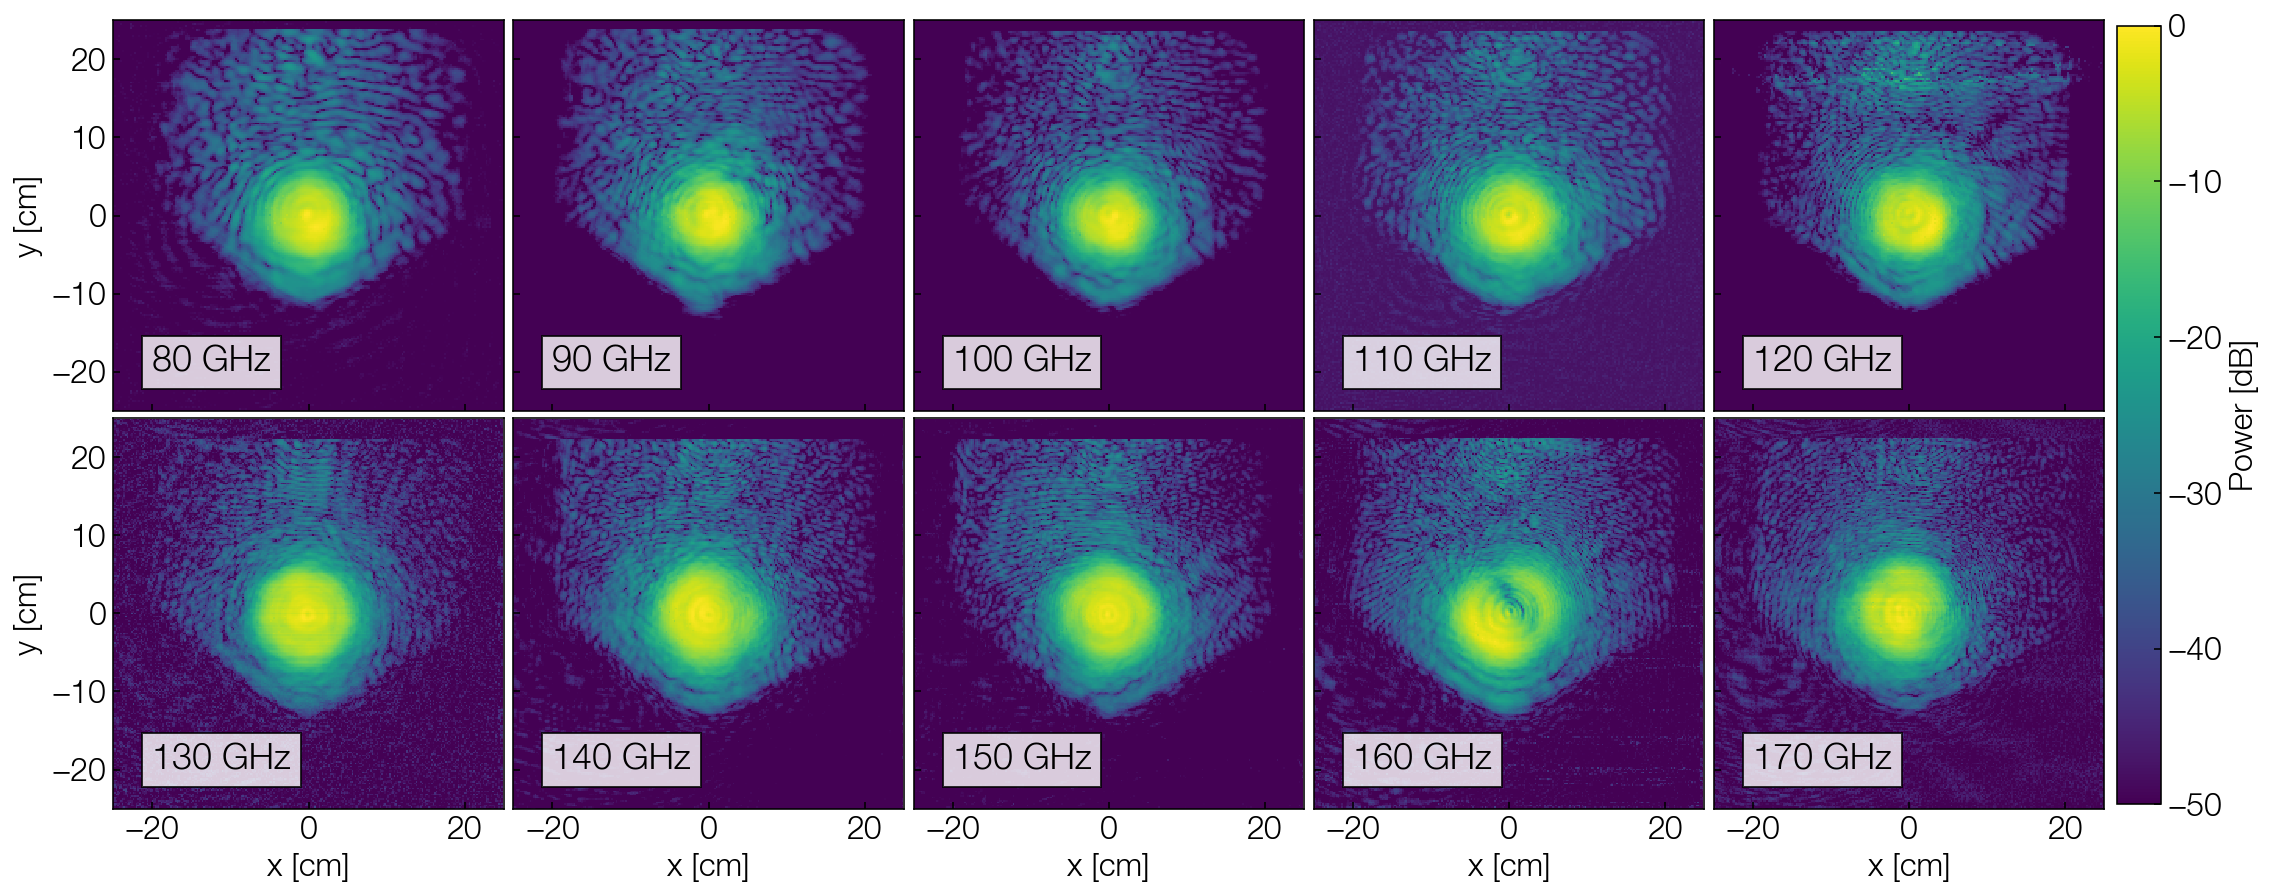
\includegraphics[width = .95\textwidth]{Figures/MF_amp.png}
    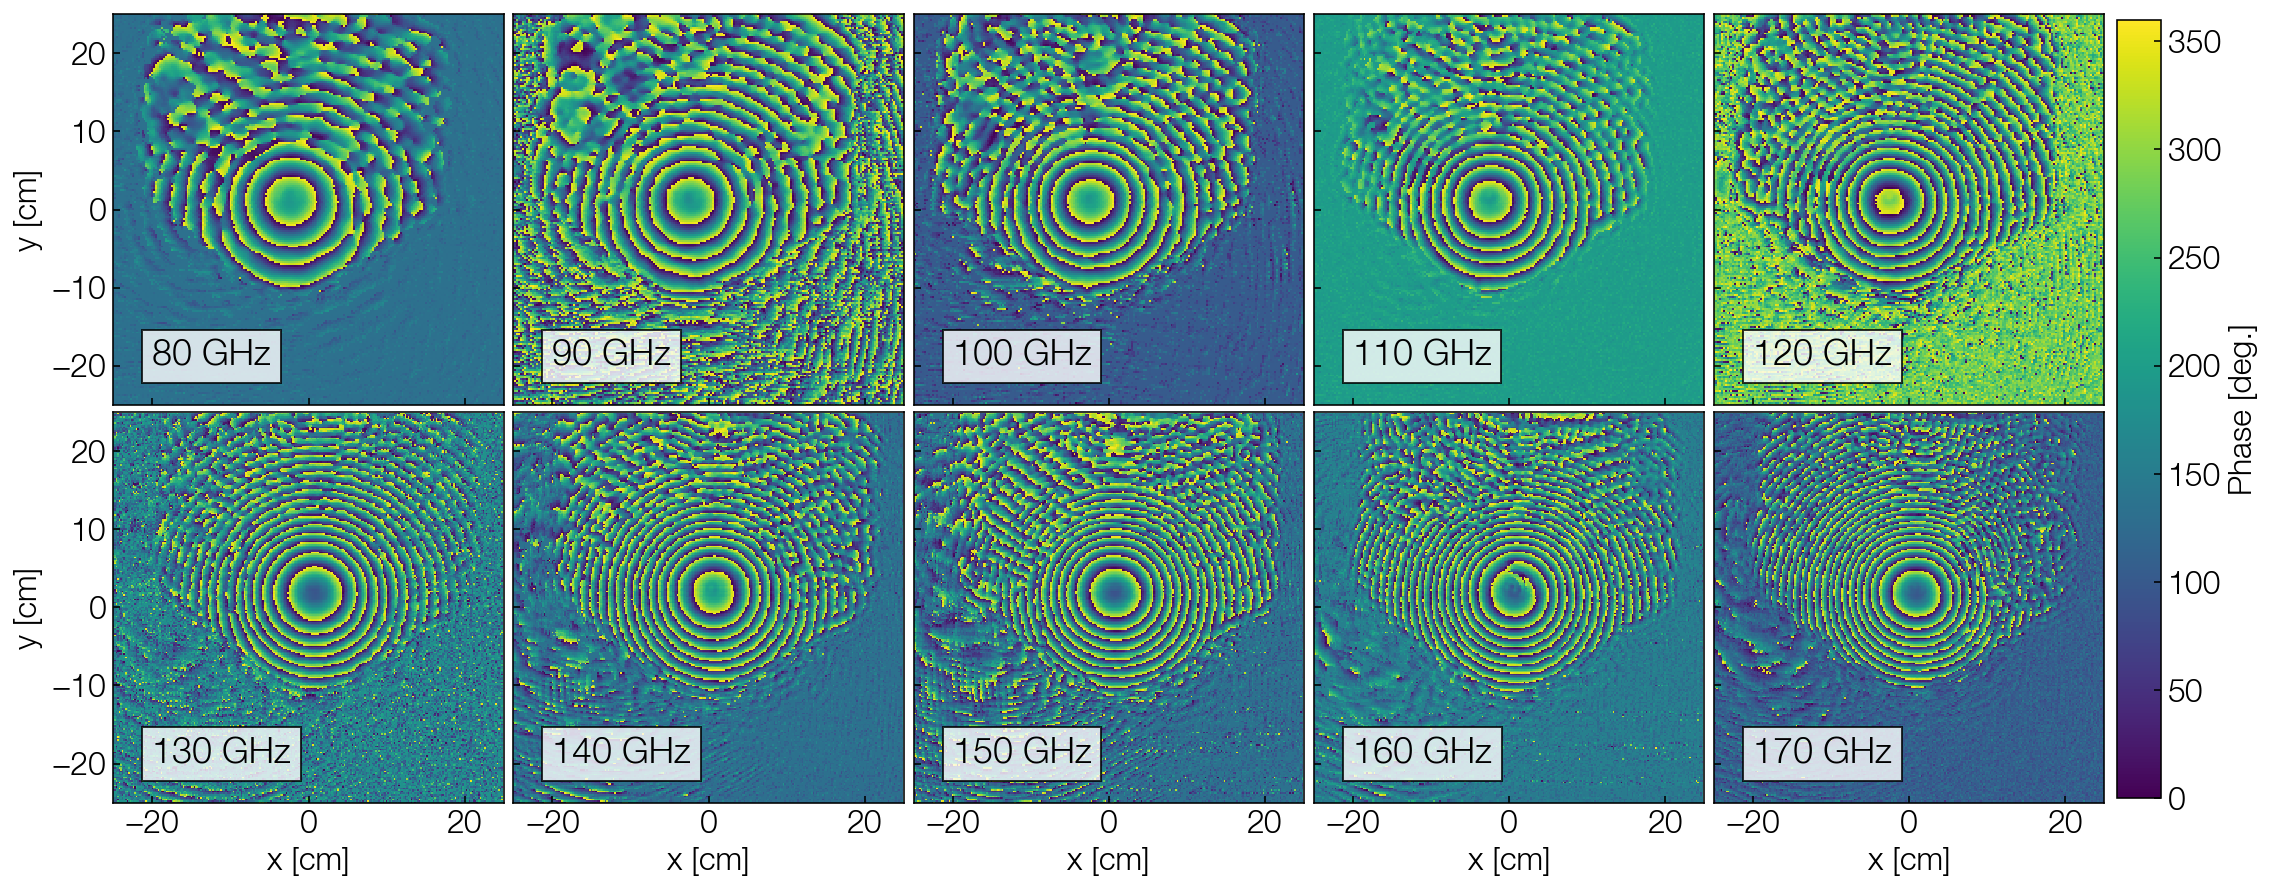
\includegraphics[width = .95\textwidth]{Figures/MF_phi.png}
    \caption{Holography beam map measurements in the mid-frequency band.  Top: Power at each measured frequency (peak-normalized in each map).  Bottom: Wrapped phase at each measured frequency.}

    \label{fig:beam_measurements_all}
\end{figure*}

\section{Results and Interpretation}
\label{sec:results}
\subsection{Near-Field Beam Maps}
Figure~\ref{fig:beam_measurements_all} shows the power and phase of the beam maps at each frequency for which the measurement was carried out.   A variable attenuator at the output of the source was used to optimize the amount of signal entering the optics tube, to ensure power was not too high such that the measurement was saturated, but to also ensure the signal was high enough for signal-to-noise greater than 45\,dB.  As stated in Section ~\ref{sec:meas_method}.\ref{sec:meas_hardware}, the F90 source hangs closer to the window than the F150 source (due to different attenuator lengths), and for this reason, we expect the F90 beams to be smaller than the F150 beams.

The shape of the main beam was found to be in good agreement with simulations at all frequencies.  The asymmetric feature seen in the main beam at 160 GHz is believed to be associated with an extra mode in the round wave-guide of the receiver.  Even with this feature, the radial profile is in very good agreement with the theoretical prediction (within 10\% at the -20dB level).   The hexagonal side-lobe seen in each beam map are associated with scattering from within the optics tube and out the hexagonal window.   The phase indicates the field of these side-lobes is diverging less quickly than that of the main beam.  

\subsection{Propagation of Fields}
\label{sec:prop_fields}

\begin{figure*}[ht]
    \centering
    \includegraphics[width = .98\textwidth]{Figures/ff_secondary.pdf}
    \caption{All beam maps propagated at the secondary illumination of the Large Aperture Telescope.  The spilled power to 300\,K is calculated by integrating power outside the boundary of the secondary (red line) with respect to total integrated power of the map.}
    \label{fig:secondary}
\end{figure*}

The performance of the LAT optical system is assessed in detail by using the amplitude and phase of the measured beams to calculate the fields as they propagate through a virtual telescope.  This enables calculation of the far-field beam of the telescope, and the amount of signal "spilled", or lost, at the LAT secondary mirror.  This represents a unique capability of holography measurements which is critical in assessing the overall performance of this system. 

\subsubsection{Fields at Secondary Illumination}
To determine the amount of power "spilled" to 300\,K, we propagate the measured fields forward and onto the plane of the secondary mirror (approximately 12\,m away from the measurement plane.  This is carried out by using the Fourier relationship between the near-field $E(x,y)$ and far-field $B(\theta_x,\theta_y)$ beams \cite{McIntosh2016,alma_holog}:

\begin{equation}
    B(\theta_x,\theta_y) = \int_{\text{aperture}} E(x,y) e^{ i \frac{2\pi}{\lambda} (\theta_x x + \theta_y y )} dx dy 
\end{equation}
where the complex electric field $E(x,y)$ is integrated over the area of the aperture, and $\lambda$ is the wavelength.

Figure~\ref{fig:secondary} shows beam maps propagated to the secondary mirror of the LAT, with the boundary  of the secondary mirror in red.  To quantify the spilled power, we integrate the power outside the boundary, and then normalize to the total integrated power of the beam map.  We find the average spilled power in the F90(150) detector band is 0.65 (0.68)\% with no significant frequency dependence.  This is below the design target of 1\% and indicates the sensitivity of SO should not be compromised by spilled power to 300\,K. 

\subsubsection{Far-Fields}

To propagate the measured near-fields into the far-field, we use a virtual telescope to produce the fields from a distant (100\,km) point source on the measurement plane.  We then multiply this field with the measured near-field beam in the corresponding plane.  Integrating the resulting field over the area of the focal plane produces the amplitude and phase of the far-field at that point.  We then rotate the telescope in azimuth and elevation and repeat this process to produce a full beam map in the sky.

\begin{figure*}[t]
    \centering
    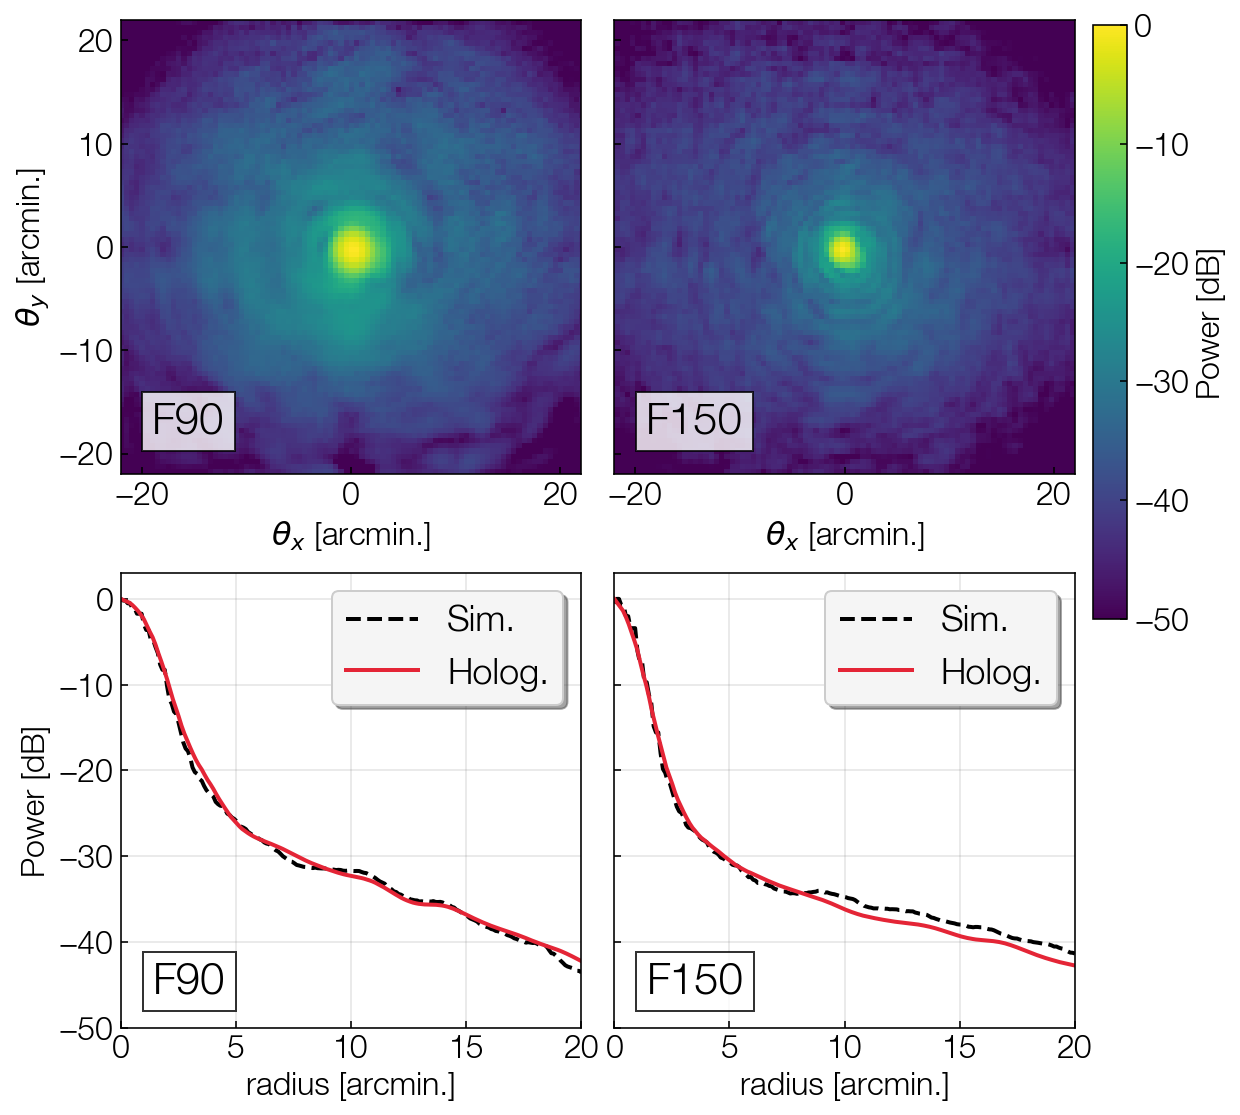
\includegraphics[width = .8\textwidth]{Figures/farfield1d.png}
    \caption{Top row: Using FD, the LATRt measurements are propagated through the LAT from the near-focal plane, to the far-field.  Bottom row: Radial profile of the measured(simulated) far-field beams in the F90 and F150 bands, plotted in red(black).}
    \label{fig:farfields}
\end{figure*}

The holography source emits its signal out of a rectangular feedhorn with a finite size.  The resulting near-field beam is convolved by this rectangular aperture~\cite{2005ifo..book.....G}.  Interpreting this measurement requires accounting for this effect, which amounts to a convolution of the electromagnetic field from the optics tube with the field pattern on the aperture of the feedhorn.  The impact of this convolution is to broaden the F90(150) far-field beam by 12.2(4.7)\% and to create square diffraction spikes in the raw far-field calculation~\cite{2005ifo..book.....G}.

We account for this effect with forward modeling, which is described in Appendix~\ref{app:holog}.  To fully simulate the far-field beam of the LAT including the optics tube, we first simulate the optics tube using \verb|solat-optics| as described in~\cite{holog_sim_model}.  This produces the near-field beam at the front of the optics tube, which is then propagated into the far-field the same way the measured near-field beams are propagated through the virtual telescope.  The resulting far-fields after diffraction spike removal are shown in Figure~\ref{fig:farfields}.  These plots are band averaged, including data from 80-110\,GHz in the F90 band and 130-170\,GHz in the F150 band.  The radial binned far-field holography data are compared to simulations.  These comparisons show that the holography data are consistent with the predicted F90(150) FWHM is 2.18(1.38) arcmin and with low ellipticity with no unexpected features such as the "little-buddies" seen in the ACTPol experiment \cite{2021arXiv211212226L,Gudmundsson:21}.

\section{Filter Removal}
\label{sec:filter}
We have described the holography results from the final instrument configuration.  However, in the initial SO configuration, which contained an additional filter (1K Low-Pass Edge (LPE) filter in Figure~\ref{fig:latrt}), we found extra signal outside the main beam from the window (hexagon at ~-20dB) at all frequencies.  While these side-lobes did not significantly change the spilled power to 300\,K, they would have reduced optical efficiency and led to an enhancement of near side-lobes of the on-sky beam.

To study the frequency dependence of side-lobe power, we computed the integrated fractional power outside the main beam.  We define the main beam radius as $13.5$\,cm, where the beam drops below -20\,dB.   Figure~\ref{fig:filter_info}B shows the integrated fractional power outside the main beam as a function of frequency, and also the measured reflectivity of the 1\,K 6.8\,cm$^{-1}$ LPE filter~\cite{10.1117/12.673162}.

\begin{figure*}[t]
    \centering
    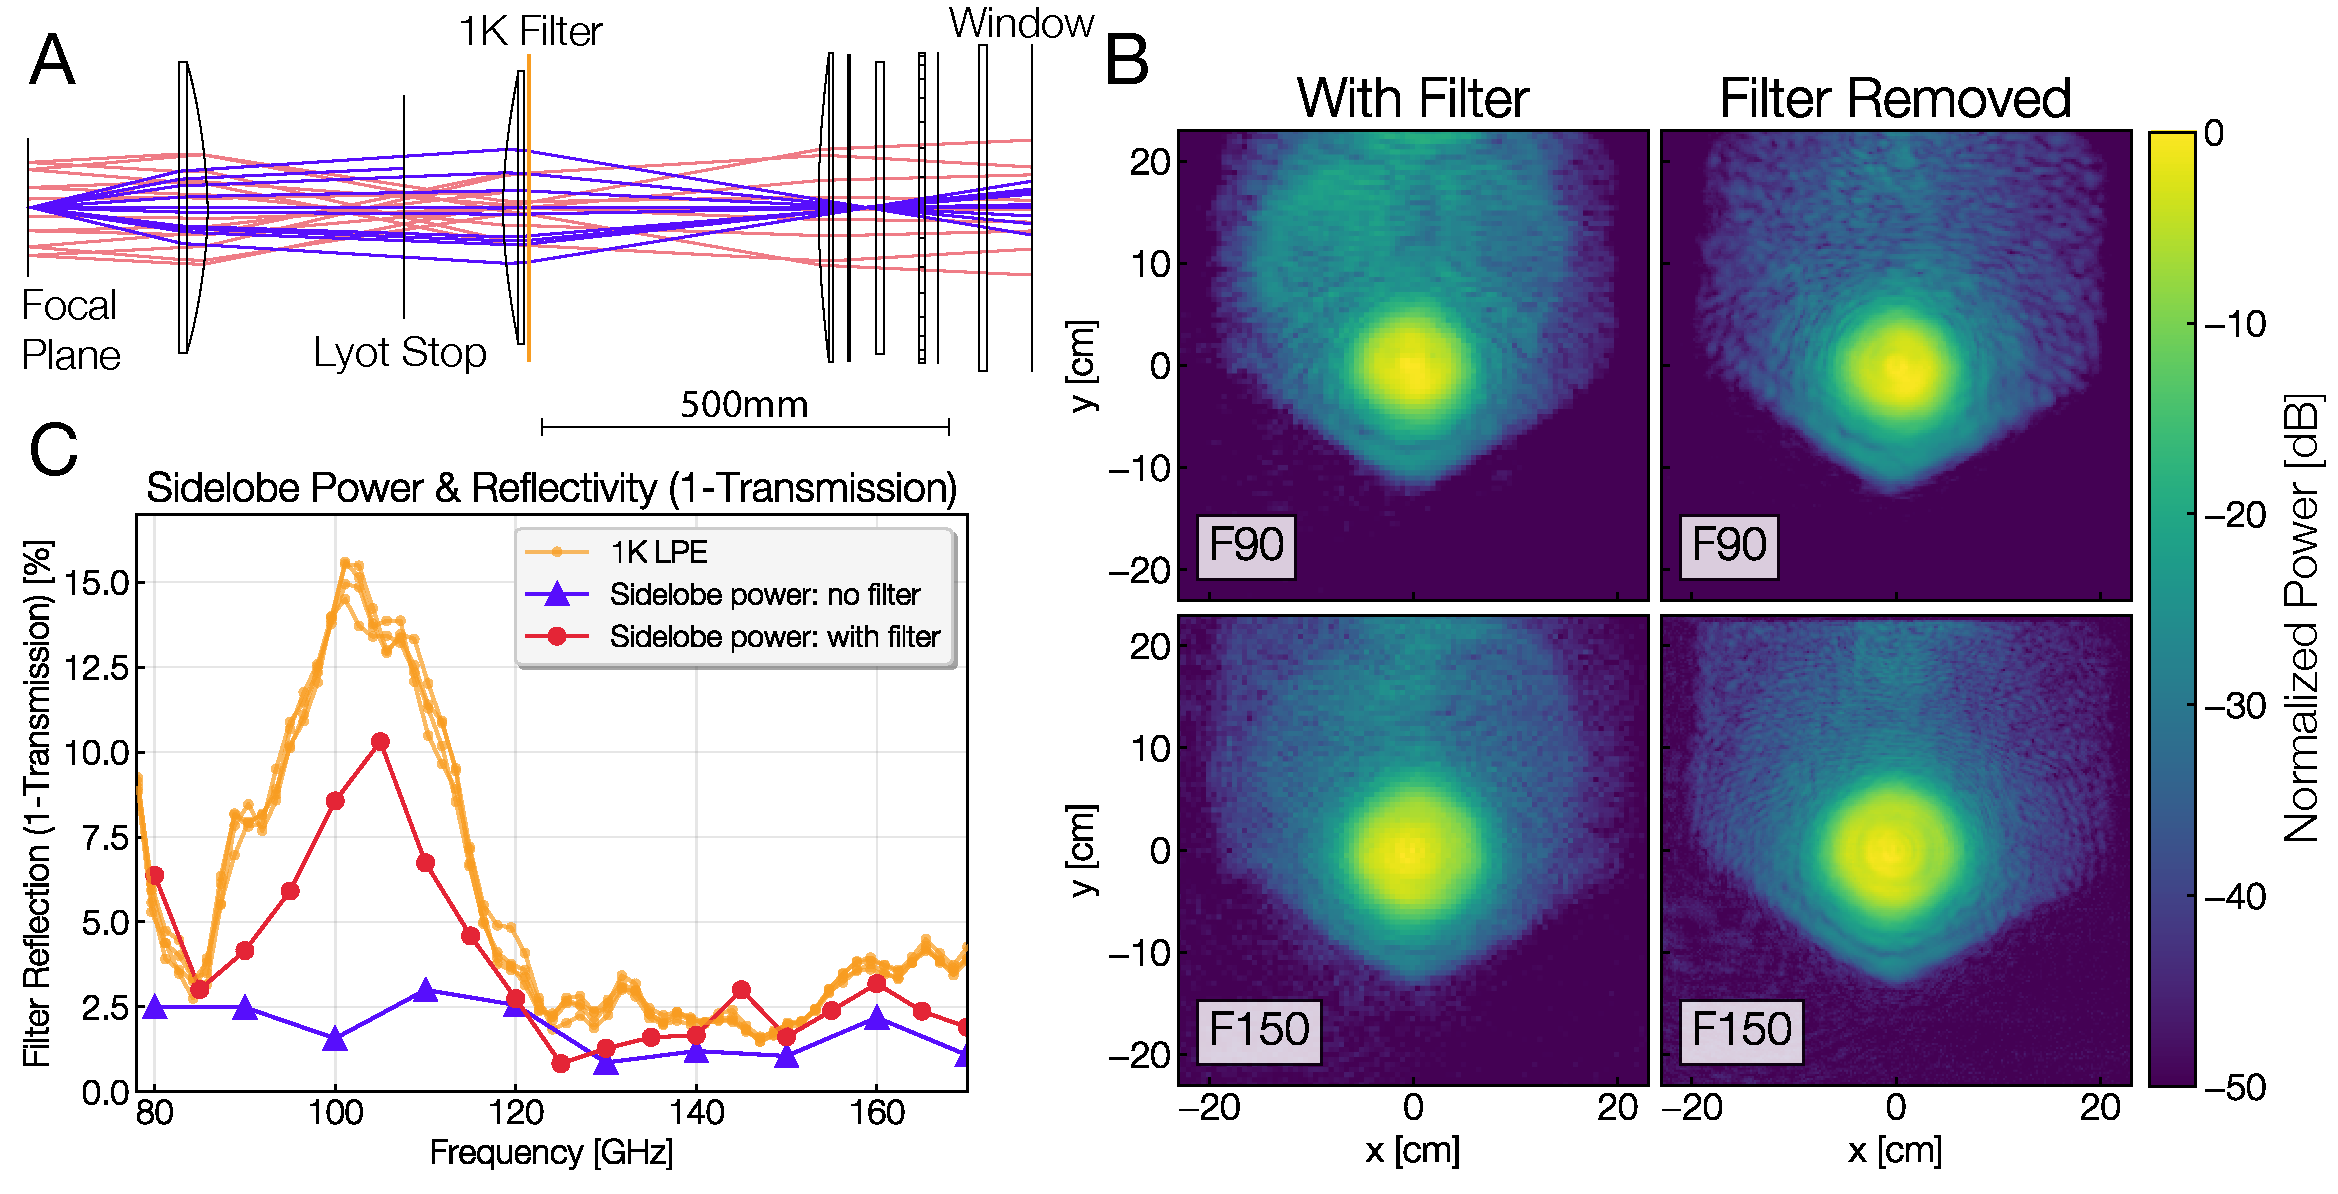
\includegraphics[width = .95\textwidth]{Figures/filter_fig.pdf}
    \caption{A) Time-reversed ray-trace of the SO LAT Optics Tube (OT) with one filter (orange), near the second lens.  With 0\% on-axis reflectivity of the filter, rays(blue) emerge from the focal plane and exit the OT window.  With an on-axis reflectivity of 5.64\,\% (average LPE filter reflectivity in the full band), rays reflected off of the filter(red) go back to the reflective focal plane (copper and reflective), and then propagate out the front of the window.  This is verified in the simulation, as the main beam in front of the OT shows the shape of the focal plane at -25\,dB.  \,\,B) In orange is the measured reflectivity (1-transmission) of the 6.8\,cm$^{-1}$ LPE filter, which is placed at the 1-K stage in the optics tube.  The red(blue) line shows the measured integrated fractional power outside the main beam at each frequency with(without) the filter in the optics tube.  \,\,C) Band-averaged near-field beam maps with and without the filter in the optics tube.  With the filter, beam maps show extra scattering in the top parts of the map, through the upper portion of the LATRt hexagonal window (hexagonal power around the main beam at roughly -20\,dB due to reflection).}
    \label{fig:filter_info}
\end{figure*}

Comparing the side-lobe power to the reflectivity measurements of all filters in the optics tube, we noticed the closest resemblance to the 1\,K LPE filter.  To investigate the effect of a reflective 1\,K LPE filter, a simulation in Zemax~\cite{zeemax} shows the expected measured signal due to reflectivity of a filter (Fig. ~\ref{fig:filter_info}A).  The simulation predicts that rays are reflected off the filter and end up outside the main beam as the rays exit the LATRt window.

After removing the LPE filter from the optics tube and repeating the holography measurements, we measured a decrease in side-lobe power.  Figure~\ref{fig:filter_info}C shows the reduced near-field side-lobe power following the removal of the filter, and the comparison of the side-lobe power with the filter in place.  With the filter removed, the new side-lobe fractional power across the band is 1.9\%, a factor of 3 lower.   The tests presented above do not include this filter.  This provides a concrete example of how holography measurements can be used to optimize cryogenic optical systems.
  
\section{Cross-Polarization}
\label{sec:crosspol}
we measure the polarization performance of the optics tube.  When the source and receiver are aligned, the source emits the TM mode out of the rectangular waveguide, which is measured at the back of the optics tube.  To modulate the polarization of the signal entering the optics tube, we use a polarization grid[CITE GRID ARTICLE].  The grid is made of.... 

We measure the polarized signal for a co- and cross-polarized source.  The co-polar source outputs a TM-mode aligned to the harmonic mixer's waveguide in the focal plane.  We attach a $90^{\circ}$ twist waveguide such that the source's TM output is perpendicular to the harmonic mixer's waveguide.

The model outputs the predicted Stokes parameters received at the back of the optics tube.  Additionally, the receiver is already slightly clocked off of perfect alignment from the source, since the tester-array required slightly tilted holes to mount the receiver.  Therefore, we include this in our polarization model.  We find a degeneracy between the instrument polarization parameters and therefor exclude them in the fit.  We conclude that the holography polarization data is insufficient to quantify the instrument polarization.  

Figure~\ref{fig:holo_crosspol_params} shows the measured power (co- and cross-polarized) as a function of grid tilt, for both co- and cross-polarized sources.  We measure the received power at 85-120\,GHz in 5\,GHz increments, and at grid tilts from 0-360$^{\circ}$, in $10^{\circ}$ increments.  From the data, we use an MCMC to constrain the detector tilt $\theta_{\text{det}}$, grid efficiency $\eta_{\text{grid}}$, and cross polarization $CP$.

Figure~\ref{fig:holo_crosspol_params} shows the constrained parameters obtained by fitting the holography polarization data to the model (Eq.~\ref{eq:holo_model}).  The detector angle $\theta_{\text{det}}$ is constrained to $-30.62^{\circ\,+0.69}_{-0.67}$, the grid efficiency $\eta_{\text{grid}}$ is constrained to $97.00\%^{+0.21}_{-0.22}$, and the cross polarization $CP$ less than $1\%$.  The source emits a polarized signal, which is then additionally polarized by the grid.  For this reason, the holography data cannot constrain the instrument polarization.  We omit the instrument polarization from the model when fitting the holography polarization data. 

\begin{figure*}
    \centering
    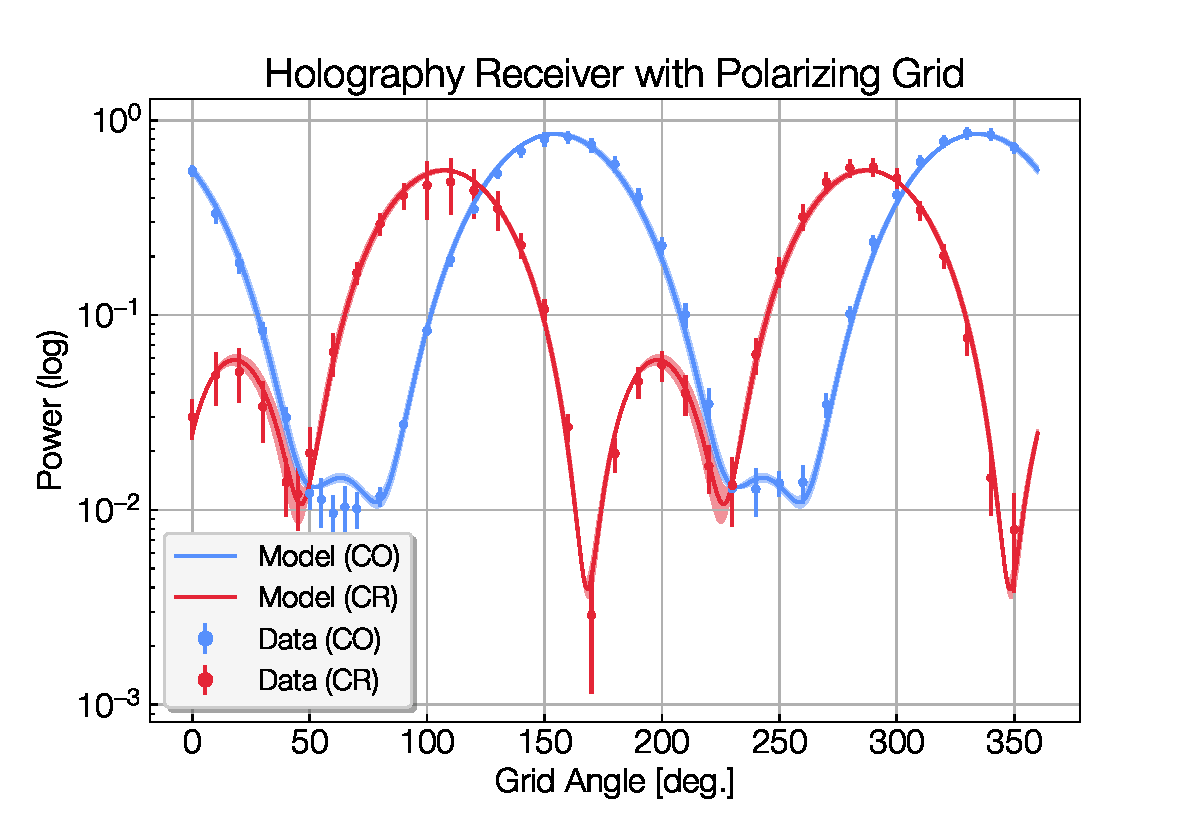
\includegraphics[height = .4\textwidth]{Figures/holo_pol_data.pdf}
    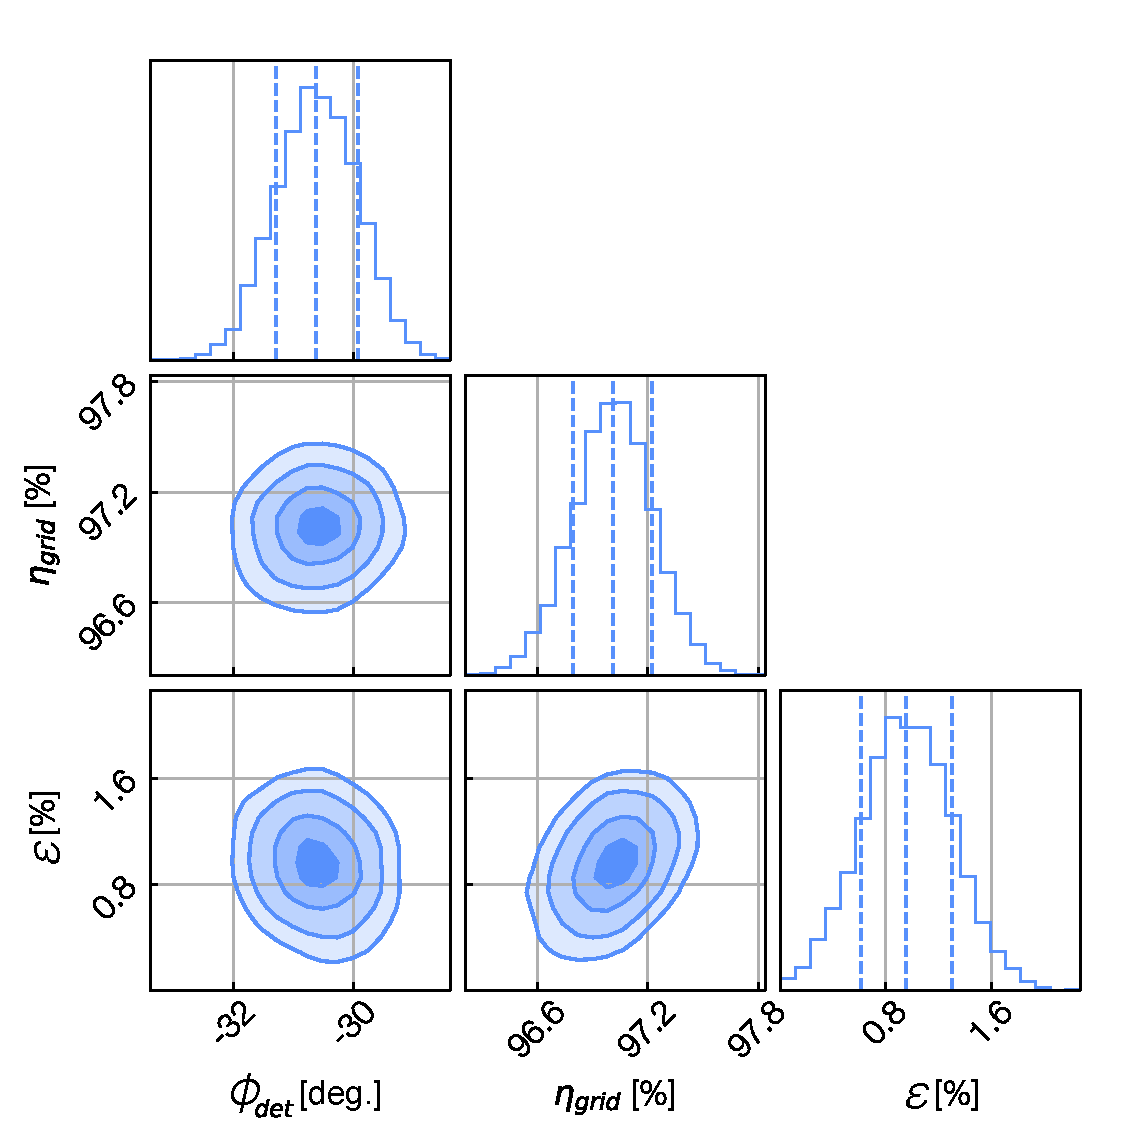
\includegraphics[height = .4\textwidth]{Figures/holo_crosspol_params.pdf}
    \caption{Left: Constrained parameters from polarization model (Eq.~\ref{eq:holo_model}), detector angle $\theta_{\text{det}}$, grid efficiency $\eta_{\text{grid}}$, and cross polarization $CP$.  Right: Polarized beam power (band-averaged from 85-120\,GHz) as a function of grid rotation, measured with the holography setup described in Section~\ref{sec:latot_meas_method}.  Co-polarization\,(blue) holds the source waveguide aligned with the receiver orientation.  Cross-polarization\,(green) uses a $90^{\circ}$ waveguide to make the source aligned perpendicular to the receiver orientation.  The polarization model (Eq.~\ref{eq:holo_model}) is fit using an MCMC and with no instrument polarization.}
    \label{fig:holo_crosspol_params}
\end{figure*}

\section{Public Code}
\label{sec:solat_code}
Here, we describe the software used for the holography data acquisition and analysis, all of which are made public.  The software is two-fold; 1) the \verb|solat-optics| module for simulating the near- and far-fields of the LAT telescope from the LATRt holography measurements and 2) Open Source Holography: a website detailing software and hardware to replicate the holography measurements.

\subsection{Optics Simulation}
The \verb|solat-optics| code includes several modules: beam simulation of the LATR optics tube, propagation of measured fields to the secondary mirror, and to the far-field (dependencies:~\cite{2020NumPy-Array,2020SciPy-NMeth,hunter2007matplotlib,reback2020pandas,mpiPython,tqdm}).  This beam simulation includes the lens geometry and computes the beam in the near-field.  The code can be adapted to produce the beam as a function of angle, as was used in this paper, or as a function of position in the measurement plane.  

The propagation analysis code inverts complex beams either from simulations or holography data, corrects for near-field aberrations using ray tracing and returns the complex fields propagated to a desired plane, either near- or far-field.   Notebooks are provided to show how to compute a beam simulation, how to analyze a LATRt holography measurement, and how to propagate a measurement to a desired region.  We invite users to adapt this code to any applications they see fit, but ask that publications using this code cite this paper and that code derived from this work remain public.

\subsection{Open Source Holography}
We also provide an open-source holography GitHub website:  \verb|holog-exp|~\cite{holog-exp}.  The repository provides both hardware and software details for recreating the holography measurements in this paper, and details on how to adapt the setup for future experiments.  The scripts demonstrate how to correlate signals with the FPGA, program the synthesizers, and program the XY stages to produce a holography beam map.  Further details can be found in Appendix~\ref{app:holog}.

\section{Conclusion}
\label{sec:discussion}
Refractive holography enables the testing of optical performance prior to deployment, and propagating the measurements into the far-field to predict the beam of the telescope.  We have presented holography measurements of the SO LAT optics tube and analysis methods determining its optical performance, including open-source holography for repeating and adapting the experiment.  We further provide an open-source package for simulating near-field holography measurements and propagating the measurements into the far-field using FD. 

From these data, we characterize the optical performance of the LATR optics tube.  We compare near- and far-field measurements to simulations.  After propagating the beams to the plane of the LAT secondary mirror, we find sub-percent power spilled to 300\,K.  We further find the far-field measured beams to be 2.18(1.38) arcmin FWHM in the F90(F150) band.

We provide three open-source software packages.  The first developed for this work, (\verb|solat-optics|~\cite{holog_sim_model}), models the LATRt holography measurements and is customizable to include arbitrary optics and adaptable for other optics experiments.  The second, (\verb|holog-exp|~\cite{holog-exp}), details the hardware and data acquisition software required in this experiment.  And lastly, we publish the data and Python scripts for recreating all figures in this paper~\cite{knowledge}.

The approach demonstrated here is broadly applicable to the characterization of millimeter-wave optical systems.  The ability to characterize the optical performance and systematics of the optics tube allowed us to determine one source of spurious reflections, and avoid systematics during future observations.  

\chapter{HoloSim-ML: machine learning applied to the efficient analysis of radio holography measurements of complex optical systems}
\label{ch:holosim}
\section{Introduction}
Simons Observatory (SO) is an ensemble of millimeter-wave telescopes which will observe the cosmic microwave background (CMB) temperature and polarization signals~\cite{gali18, so19}. SO comprises one Large Aperture Telescope (LAT)~\cite{Niemack:16, Gudmundsson:21,Parshley_2018} and three Small Aperture Telescopes (SAT)~\cite{ali20} which together will measure the temperature and polarization anisotropy of the CMB from several degrees to arc-minute angular scales.

The science goals of SO require high sensitivity and tight control over systematic errors.  Since the sensitivity of state of the art millimeter-wave receivers is limited by photon noise from background radiation, improvements in sensitivity for a given instrument require careful control over every part of the instrument.  Deviations of the mirror surface will redistribute beam power to large angular scales and therefore increase the width of the main beam and reduce the forward gain of the telescope.  In this work we focus on quantifying these effects, and we present the tools needed to mitigate them by aligning the mirror panels of the LAT using holography.

The LAT is a crossed-Dragone telescope~\cite{6773968,Gudmundsson:21,Niemack:16,2021RNAAS...5..100X} developed in collaboration with the Cerro Chajnantor Atacama Telescope prime (CCAT-prime)~\cite{ccat,aravena2019ccatprime} Collaboration.  The LAT design is shown in Figure~\ref{fig:lat}.  The telescope is engineered and built by Vertex Antennentechnik GmbH, the panels forming the primary and secondary mirrors, both 6 m in diameter, were fabricated by Bricon Technology GmbH~\cite{vertex}.  A defining feature of this design is the large focal plane (2\,m in diameter) that can accommodate more than 70,000 detectors for CMB studies~\cite{Parshley_2018,zhu2021simons,mccarrick2021simons}. The primary\,(secondary) mirror is built with 77\,(69) panels, and has 385\,(345) adjusters in total.  The size of each panel is roughly half a square meter and weighs roughly 5\,kg~\cite{ccat}.  An adjuster is a threaded mechanism allowing for manual adjustment of the position of each panel~\cite{Woody}.  Each panel has five adjusters controlling the surface height.  We present radio holography tools that allow us to reach a combined reflector surface error of $22\,\mu$m RMS or less.

Radio holography has a long history of use in millimeter and sub-millimeter telescopes~\cite{alma_holog,Sridharan,7228408,5722985,morris:1143663,Fienup:93}.  Typically, these applications require aligning a single mirror, which can be measured in isolation~\cite{1141354,Hunter2011}.  A particular challenge of this application is that we must measure both mirrors simultaneously and then extract the adjuster errors from each of the two mirrors.  This complex optical system requires the development of new fitting tools for efficient analysis.  Towards this end, we developed an efficient simulation code and used it to train a machine learning (ML) model to do this extraction.
Practical holography measurements of telescopes of this size must be carried out with a bright monochromatic source in the near-field.  The analysis of near-field holography is described in great detail in several references~\cite{alma_holog,5722985,1190}.  The CCAT-prime Collaboration carried out a parallel work simultaneously with ours, which details measurement methods \cite{fyst_holog}.  The method described is commonly referred to as “near-field vector beam mapping” and employs a coherent source and phase sensitive receivers.  For a given desired accuracy, this requires a lower signal-to-noise than Out-of-Focus Holography (OFH), which reconstructs the telescope aperture phase through comparison of far-field power maps taken in and out of focus with a coherent source and incoherent detectors in the focal plane~\cite{Serabyn:91}.  In this work, we examine the impact of mirror alignment on measurements of the CMB, explore the sampling of the focal plane required to arrive at a given mirror RMS, and  present a new approach to fitting complex optical systems that we expect to be far more general than the present example.

In Section~\ref{sec:motive} we quantify the scientific impact of improving the mirror surface.  In Section~\ref{sec:simulate} we describe the simulations we use to model these holography measurements.  In Section~\ref{sec:method_align} we describe our analysis of near field holography data using ray-tracing to determine the near field corrections.  In Section~\ref{sec:ml} we describe how we use these simulations to train a machine learning code to efficiently and accurately extract the adjuster errors from holography data.  We discuss how the number of measurement positions impacts the remaining degeneracies in the panel errors.  In Section~\ref{sec:meas_method} we explain the method for performing this measurement, including hardware tolerances and alignment.  Section~\ref{sec:code} details the publicly available code.  We conclude with a discussion of other potential applications in Section~\ref{sec:holosim_conclusion}.  
\section{Motivation}
\label{sec:motive}

Measurements of the CMB are typically expressed as power spectra computed from all-sky maps using the spherical harmonic transform.  Therefore, the impact of the scattering of power due to mirror surface deviations can be understood by transforming these beams into $\ell$-space window functions.  These window functions encode how the beam shape rolls off the CMB power spectrum as a function of $\ell \sim 180^\circ / \theta$.  This transformation is equivalent, in the flat sky limit, to Fourier transforming the beam and averaging its magnitude squared in bins of constant wave number.  For reference, $\ell = 1000$ corresponds to an angular scale of $0.18^\circ$.

\begin{figure}[t]
    \centering
    \includegraphics[width = .7\textwidth]{Figures/far_field_win_func2.pdf}
    \caption{Top: Far-field beam simulation of a 150 GHz source, with surface error RMS of $0\,\mu$m, $20\,\mu$m, $35\,\mu$m, and $50\,\mu$m. The side-lobes around the central beam increase as RMS of panel errors increases. Center: Window function $W_\ell$ of far-field beams at 150 GHz with combined surface RMS of $50\,\mu$m, $35\,\mu$m, $20\,\mu$m, and $0\,\mu$m. Bottom: Difference of window functions $W_\ell$ in top plot, w.r.t. window function of far-field beam with surface error RMS of $0\,\mu$m, $W_{\ell,0\mu}$.}
    \label{fig:win_func}
\end{figure}
The upper panels of figure~\ref{fig:win_func} show simulations of the LAT beam pattern with varying levels of panel setting errors at 150 GHz, one of our key science bands.  These simulations were generated using the method described in Section~\ref{sec:simulate} in the far-field.  We note that the calculation extends to a larger angle, but we have truncated it in the figure for clarity of presentation.  It is apparent that the panel errors lead to significant scattering of light from the main beam into near side-lobes.

The plots of Figure~\ref{fig:win_func} display these window functions for the simulated beams (top row) and the difference between the window functions with panel errors and that of a perfect mirror (bottom).  For reference, the vendor will deliver the telescope mirrors with a half-wave front error (HWFE) of $50\,\mu$m.  The current method of panel alignment using a laser tracker achieved a surface error of the panels to $20-25\,\mu  m$ for the 6\,m primary mirror of the Atacama Cosmology Telescope~\cite{act_inst}.  The surface error budget for the SO LAT give a $35\,\mu$m HWFE if similar panel errors are achieved.  This leads to a 10\% loss in signal in the $1000<\ell < 5000$ range that is crucial for much of the SO science~\cite{so_science}.  This matches the prediction of the Ruze formula~\cite{ruze} once one accounts for the fact that the power spectrum (and window function) are proportional to the square of the beam.  Since the calibration of the power spectrum is based on cross-correlating with data from the Planck Satellite~\cite{planck_data} for $\ell \lesssim 1600$, the variation in the window function in this range represents a potential systematic challenge.  Reducing the half-wave front error to below 22 $\mu$m would simplify calibration and recover most of this lost sensitivity.  The error budget for our telescope shows that this requires measuring and setting each of the primary and secondary mirror to an accuracy of better than $5 \mu$m RMS, which we take as a goal for this work.

\section{Beam Simulation}
\label{sec:simulate}
The SO LAT is shown in Figure~\ref{fig:lat} and described in~\cite{2021RNAAS...5..100X}.  We compute its beam pattern in the near-field and far-field using physical optics~\cite{hecht,Gudmundsson:21} implemented in a code we call \verb|HoloSim-ML|, available at GitHub.com/McMahonCosmologyLab~\cite{McMahonCosmologyLab}.

\begin{figure}
    \centering
    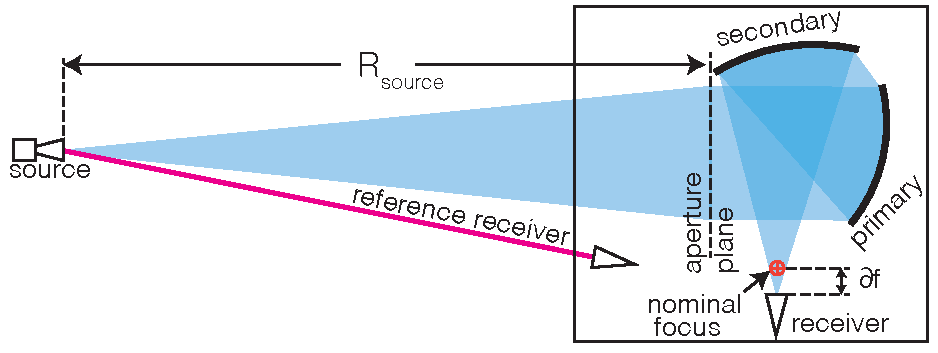
\includegraphics[width = .9\textwidth]{Figures/holography_geo3.pdf}
    \caption{Holography geometry. A source on a 5\,m tower sits at a distance $ R_{\text{source}}$ above the aperture plane of the LAT. Two receivers, one "reference" receiver pointed straight at the source, and the receiver in the focal plane, measure the amplitude and phase of the source. The focal plane receiver is offset $\delta f$ from the nominal focus.}
    \label{fig:hologeo}
\end{figure}

A two-dimensional representation of the three-dimensional geometry used in these simulations is shown in Figure~\ref{fig:hologeo}.  We specify the positions and rotational state of the mirrors, the location of the receiver feed, and the location of the source.  For these simulations, we refocus the telescope on the near-field source by displacing the receiver a distance $\delta f$ from the nominal telescope focus. We ray-trace from a receiver position through the telescope to an aperture plane chosen at an arbitrary position a few meters in front of the telescope. The results do not depend on this arbitrary choice.  Each ray is given an amplitude based on a modeled beam pattern for the receiver feed horn.  A reference receiver, placed outside the telescope, points directly at the source and, in combination with the receiver feed, determines the phase of the source.  For the results presented here, the beam width of the receiver feed was assumed to be $44^\circ$ with a Gaussian profile.  We typically use a 100\,x\,100 grid of points on the aperture plane. This telescope model is rotated, and this calculation is repeated for every azimuth and elevation pointing to simulate the two-dimensional diffraction pattern.

To model misalignment of the mirrors, the surface $z_{surf}$ of each mirror panel, is parameterized as a polynomial function of the five parameters $a_n$:
\begin{equation}
     z_{\text{surf}} = a_1 + a_2 r_x+ a_3 r_y +a_4 (r_x^2 + r_y^2) + a_5 r_x r_y 
     \label{eq:zsurf}
\end{equation}
where $r_x$ and $r_y$ are coordinates centered in each individual panel.  The $a_n$ parameters are determined by fitting this equation to the surface offsets $\delta_z$ at the positions of the five mirror adjusters. Thus, there is a one-to-one mapping between adjuster offsets and the parameters in this model.  The surface machining errors for each panel will be a few micrometers and the adjuster system is the same as was used for SPT where a similar model was fit successfully \cite{Carlstrom_2011}.  Therefore, this panel model is expected to be adequate for these purposes.

\begin{figure}[t]
    \centering
    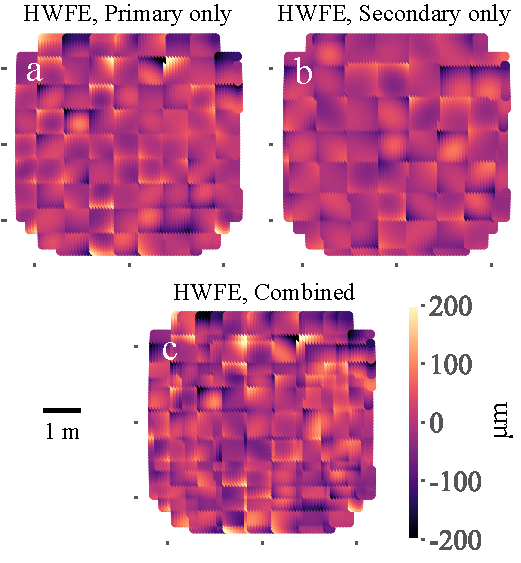
\includegraphics[width = .8\textwidth]{Figures/example_pathl_single_column2.pdf}
    \caption{Simulated HWFE at the aperture plane with surface errors of $35\,\mu$m RMS on a) only M1, b) only M2, and c) both M2 and M1.}
    \label{fig:pan_mod}
\end{figure}

The output of this step in the code is the amplitude and path length to the aperture plane from the receiver feed.  Figure~\ref{fig:pan_mod} shows the resulting variation in the path length across the aperture plane for one realization of panel errors from the primary mirror (left) to the secondary mirror (right) and the combination of both (bottom).  It is clear that the errors due to the secondary and primary mirror panel misalignments occur at slightly different physical positions and scales in the aperture plane.  This means that a single holography measurement may suffice to extract the panel errors. 

The next step in the calculation is to determine the straight line path length from each point in the aperture plane to a source.  The source is chosen to be at $R=1\times 10^6$\,m for the far-field and $R=1\times 10^3$\,m for near-field holography.  The elevation $\theta$ and cross-elevation $\phi$ of this source are varied to map out the beam.  This results in a total path length from the source to the receiver.  The beam $B(\theta,\phi)$ is then calculated using:
\begin{equation}
    B(\theta,\phi) = \sum_j E_j e^{i \rho_j(\theta,\phi) 2\pi/\lambda} 
\end{equation}
where $j$ is an index for the rays in the simulation, $E_j$ is the electric field amplitude of a ray, and $\rho_j(\theta,\phi)$ is the path-length from receiver through the telescope and to the source tower for a given pointing, and $\lambda$ is the wavelength.  We note that we can also compute the diffraction pattern in the aperture plane by fixing the source's position and varying the receiver position in the focal plane.  

\label{sec:method_align}
Radio holography consists of measuring the electric field amplitude and phase of the beam, and then utilizing the Fourier transform relationship between the aperture fields and beam to extract the fields and phase on the aperture plane.  In our case, variations in the phase of the aperture plane are interpreted as two times the errors in the mirror surface.

For practical reasons, and to reduce the impact of atmospheric turbulence, these measurements are usually carried out with a near-field transmitter.  This introduces de-focus and other geometrical aberrations that must be removed in order to interpret these data.  In previous analyses, these have been corrected by fitting out functional forms that capture these effects~\cite{alma_holog}.  Here we use our ray tracing code to model the aberrations by computing the phase on the aperture plane, including contributions internal to the telescope and between the telescope and the source.  This requires that we measure the position of the source and the position of the receiver.  After we apply this phase correction, we also remove a constant and gradients from the aperture fields to account for any small pointing errors.  This approach has been checked against the standard series expansion and generalizes easily to include additional corrections, including for the phase of the receiver feed horn.  The left panel of Figure~\ref{fig:ap_resids} shows the simulated holography measurement of SO that results from this calculation.

\section{Panel Fitting with Machine Learning}
\label{sec:ml}
To extract the adjuster offsets from the aperture field, we must simultaneously fit a model of all panels on both mirrors, including the geometric effects of the telescope.  While standard fit techniques can work, they are slow to converge and often yield solutions that are suboptimal in the sense that they under fit the panel errors.  This results in a situation where many cycles of holography measurement and analysis are required to correctly set the mirror surface.

\begin{figure}[t]
    \centering
    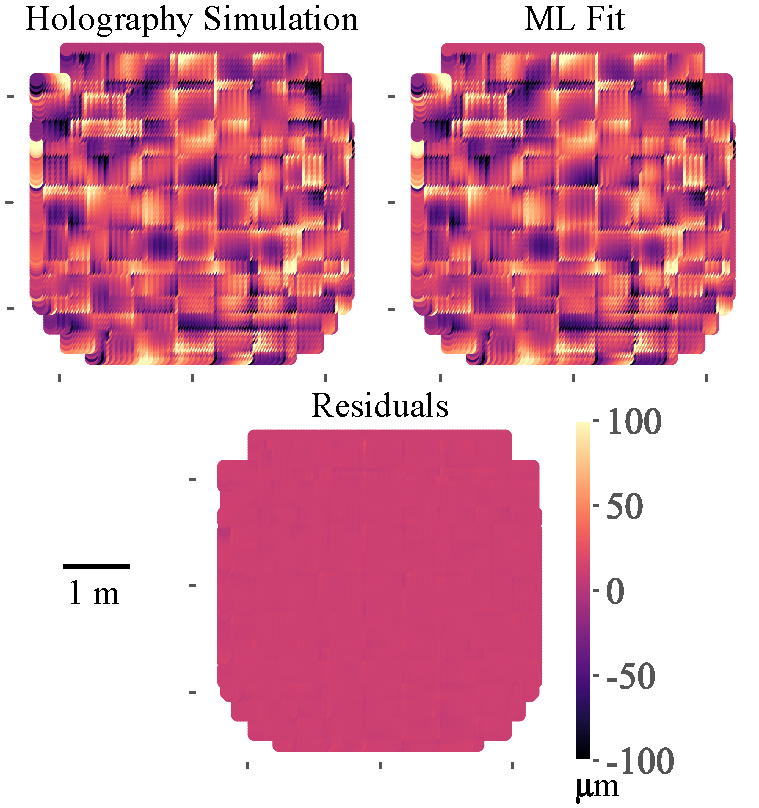
\includegraphics[width=.8\textwidth]{Figures/ap_length_corrected_single_pannel3.pdf}
    \caption{Results from simulation.  The top left panel shows the input simulation, which had 35 micrometer RMS HWFE.  The top right panel shows the predicted aperture phase given the ML determined estimates for the panel errors, and the bottom shows the residuals.}
    \label{fig:ap_resids}
\end{figure}
Here, we use a machine learning model built from the \verb|scikit-learn| python package~\cite{scikit}. To train this model, we generate a set of 1000 near-field beam simulations, each with a different realization of mirror setting errors.  Each beam simulation assumes an angular width of 200 arcmin., with 1 arcmin. spacing, for a total of 40,000 points in a 2d grid.  We then perform the holography analysis described above to yield a simulated data set comprised of aperture fields and the known input adjuster errors.  This suite of simulation is used to train a linear regression model.  The training took only minutes on a laptop, making the beam simulations the limiting computational step.  Once trained, this model will transform an input holography measurement into a set of estimated panel adjuster offsets.

Figure~\ref{fig:ap_resids} shows the results from a simulation.  The top left panel shows the input simulation, which had $35\,\mu$m RMS HWFE.  The top right panel shows the predicted aperture phase given the ML determined estimates for the panel adjuster positions, and the bottom shows the residuals.  An impressive feature of ML is that it achieved residuals below $3\,\mu$m for the combined HWFE for each of the 10 randomly chosen input simulations we tested.

\begin{figure}[t!]
    \centering
    \includegraphics[width=.9\textwidth]{Figures/m1m2_degeneracies.pdf}
    \caption{The left and middle columns show the surface errors on the Primary and Secondary mirrors after holography has been used to correct the mirror surfaces.  The right column shows the HWFE as a function of focal plane position.  The top row shows results for holography taken at a single position (see red dot).  The middle row shows results for binocular holography (combining measurements from two positions, see red dots).  The bottom row shows results for trinocular holography (combining measurements from three positions, see red dots).}
    \label{fig:m1m2_errs}
\end{figure}

One issue is that this fit is degenerate, in the sense that anti-correlated errors on the primary and secondary can cancel when measured from a single feed position.  To explore this, we plot the errors on the Primary and Secondary in Figure~\ref{fig:m1m2_errs}.  We also compute the half-wave front error on the aperture plane as a function of feed position across the large 2\,m focal plane used by SO to explore how the cancellation of this degeneracy varies with position.  The top row considers holography taken in the classical way with a single receiver position.  The middle row considers binocular holography, where two measurements taken at two positions are analyzed jointly to break degeneracies.  The bottom row further considers trinocular holography, where three measurements taken at three positions are analyzed jointly to further break degeneracies. 

These results show that standard single receiver holography leads to anti-correlated errors of $10\,\mu$m on each mirror, which cancel to less than $6\,\mu$m over most of a 2\,m focal plane.  The binocular results improve the mirror residuals to $6.5 \,\mu$m RMS, but still suffer from correlated errors that lead to HWFE marginally worse than for the single position holography.  These are below  $6.5\,\mu$m over much of the focal plane.  

The trinocular method improves the single mirror precision to $4\,\mu$m with suppressed degeneracies  which cancel  to better than $4\,\mu$m HWFE over all but the edges of the focal plane.   We have presented these results for a single realization of mirror errors, but we repeated the calculation 10 times and found the results to be robust.  Reducing the HWFE from panel setting to be below 5 $\mu$m requires trinocular holography.


%%%%%%%%%%%%%%%%%%%%%%%
\section{Measurement Practicalities and Robustness of Method}
\label{sec:meas_method}
Achieving results at this precision requires measurement hardware and methods with sufficient sensitivity and control of systematic effects, both of which are within reach.

The simulations were informed by the geography of the SO LAT site.  A 1\,km transmitter distance was chosen since the transmitter can be placed on the slope of Cerro Toco, a nearby mountain peak, at this distance and an elevation of $10^\circ$.  Given this choice, we can determine requirements on signal-to-noise and the knowledge of the location of the transmitter and receiver with respect to the telescope by varying these in our simulations.  Table~\ref{tab:tols} presents the results of this sensitivity analysis. 

We also tested the robustness of the ML method to differences between the (simulated) measured mirror surface and the training set.  We found that for measurements of mirror surfaces significantly worse than what was in the training set, the method gracefully degrades in a way that it fits out 90\,\% of the input surface.  For example, with a 100\,$\mu$m HWFE the difference between the input and fit results had an RMS of 10\,$\mu$m.  Repeating the measurement and alignment process a second time would reduce the alignment errors below our $5\,\mu$m target. 

\begin{table}[!b]
\centering

\begin{tabular}{|l|c|}
\hline
Minimum signal-to-noise & $80$\,dB\\
\hline
receiver position (arbitrary direction) & $2$\,mm \\
\hline
Tower source (radius) & $1.2$\,m \\
\hline
\end{tabular}
\caption{Allowed variation in signal-to-noise and positional knowledge needed to keep error contributions from these effects  below $2.5\,\mu$m HWFE.}
  \label{tab:tols}
\end{table}

The signal-to-noise requirement can be met with a source consisting of a Gunn Oscillator phase locked to an Oven Controlled Crystal Oscillator (OCXO).  Such a system can output hundreds of mW with a frequency stability of a few parts per billion.  This ensures the source remains reliably within a bandwidth of a few hundred Hertz, allowing for aggressive filtering of the received signals.  With this filtering, simple receivers based on harmonic mixers (noise temperatures of 100,000\,K) can in principle achieve signal-to-noises in excess of 130\,dB.  This enables broad illumination of the telescope to make the measurement immune to the source beam pattern and reduce the received signal power to below 1\,mW, a level that comfortably guarantees the detector response is within the linear regime and ensures more than sufficient signal-to-noise.

The position knowledge of the source and receiver can be measured with a combination of metrology and fitting in the analysis code.  The distance between the tower source and the telescope can be determined to better than 1\,m using a theodolite, which is a standard surveying tool.  The angular position of the source will be found with the central peak of the beam map.  Any residual errors in this angle are mitigated by the removal of a gradient in the phase on the aperture plane in the holography analysis.  The location of the receiver relative to the mirrors can be determined using a laser tracker to better than 1\,mm.  These positions can be verified by fixing one (e.g., the source distance) and then fitting the other (e.g., the receiver positions) using our simulation code.  In this way, we can determine and confirm these distances to ensure the phase corrections are correctly applied.  

The $x$ and $y$ positions of the panels are determined by centering the measured aperture fields in the coordinates used in the simulations.  We include this centering process in our results.  Therefore, this method is robust to alignment errors.

Three remaining issues, which can produce spurious phase variations in the aperture plane, must be considered: atmospheric fluctuations, the phase of the receiver feed, and the phase stability of the reference receiver.  The choice of 88 GHz should provide sufficient stability in the Chilean atmosphere at 17,000 feet.  This will be verified with repeated measurements.  The phase as a function of angle of the receiver feed will be measured in lab using the holography source and receiver.  It is straightforward to include this correction in the modeling code to remove its impact on these measurements.  Finally, the reference receiver must receive signals from the source without being affected by spurious reflections from the ground, and the cabling from it to the correlation receiver must be phase stable over the duration of the measurement.  The first concern can be addressed by feeding the reference receiver with a relatively high gain antenna, to exclude the ground, and mounting it off of the telescope to ensure its reflections aren't modulated.  The stability concern can be addressed with a scan strategy that revisits the beam center often to allow for the removal of drifts.  This approach also provides additional suppression of atmospheric phase effects.  

This approach and these considerations are similar to what was done for ALMA~\cite{alma_holog} and SPT~\cite{Carlstrom_2011}. The desired measurement precision is not significantly different from what was achieved in these previous measurements.  The SPT alignment residuals ($16\,\mu$m), were limited by the telescope stability rather than the measurement accuracy.  The measurement would take several hours to scan over $~2^\circ$, with arcminute resolution, once all hardware is fully set up.  A measurement at the desired precision is well within reach based on the measurement concept we have presented and these previous examples.

%%%%%%%%%%%%%%%%%%%%%%%%%

\section{Public Code}
\label{sec:code}
All code used for this paper is available on GitHub under the name \verb|HoloSim-ML|. The code includes two modules: beam simulation and holography analysis with mirror panel error fitting.  This beam simulation includes the mirror geometry and panel setting errors and computes the beam in both the near- and far-field regions.  The code can be adapted to produce the beam as a function of angle, as was used in this paper, or as a function of position in the focal plane.  The later may be more appropriate for a holography measurement using the method described in~\cite{fyst_holog}. The holography analysis code inverts complex beams either from simulations or holography data, corrects for near-field aberrations using ray tracing and returns the mirror surface errors.  We also include code that determines the near-field corrections following the analytic expressions presented in~\cite{alma_holog}.  The panel fitting code uses a machine learning algorithm  trained with beam simulations.  Notebooks are provided to show how to compute a beam simulation, how to analyze holography, and how to set up and run the panel fitting.  We invite users to adapt this code to any applications they see fit, but ask that publications using this code cite this paper and that code derived from this work remain public.

\section{Conclusion}
\label{sec:holosim_conclusion}
We have presented the simulation and analysis of holography data, including the application of machine learning techniques, to recover panel adjuster errors from a complex optical system comprised of two mirrors that create partially degenerate features seen in the phase on the aperture plane.  The power of machine learning is that it enables the efficient analysis of these data to separate the contributions of each mirror with high accuracy on small angular scales.  On larger scales, this method creates degenerate solutions which can be addressed with holography from multiple receiver positions.  The ML framework makes the analysis of these measurements from many receiver positions straightforward to analyze.  We presented an example of the SO dual reflector optical system and demonstrated that this approach can yield $<5\,\mu$m alignment errors, the requirement for SO science goals.

The approach demonstrated here comprises forward modeling of an optical system, sampling the system from multiple positions in the focal plane, and the application of ML to simultaneously determine many physical parameters which encode errors in the optical system.  While a standard fitting method could also work in this application, we found that after one month of fine-tuning, we were only able to fit out half of the RMS of this dual reflector system.  The ease of setting up and fitting with these ML tools was striking, while it also improved the quality of the fits for single mirror systems.  We anticipate that this approach can be applied to a variety of complex optical systems, including systems with multiple lenses, filters, absorbers, and other optical components.  For example, the SO~\cite{gali18} system includes re-imaging optics comprising three lenses, and filters.  An immediate future application is to apply these techniques, using holography, forward modeling, and ML to understand the optical properties and interactions within the system.  With proper parameterization of the imperfections and alignment errors, combined with sampling the focal plane at several positions, we anticipate that machine learning will prove to be an increasingly important tool in the characterization and performance optimization of complex optical systems. 

This software package developed for this work (\verb|Holosim-ML|~\cite{McMahonCosmologyLab}) is customizable to include arbitrary optics while remaining simple to script.  It is possible to substitute commercial simulation software within this ML framework if necessary.  However, we chose to write a self-contained code to create an open access package that is efficient and can be widely shared.
\chapter{Title of CMB Analysis Project}

\appendix

% Appendix Template

\chapter{Appendix Title Here} % Main appendix title

\label{AppendixX} % Change X to a consecutive letter; for referencing this appendix elsewhere, use \ref{AppendixX}

Write your Appendix content here.



\bibliographystyle{unsrt}
\bibliography{thebibliography.bib}


\end{document}